% Control Engineering Practice version (Elsevier CAS, double column). First port, 2026-11-24.
% Build: tectonic -X compile main.tex
\documentclass[a4paper,fleqn]{cas-dc}

\usepackage[authoryear,longnamesfirst]{natbib}
\usepackage{amsmath,amssymb,amsthm}
\usepackage{booktabs,array}
\usepackage{enumitem}
\usepackage{xcolor}
\usepackage{microtype}
\usepackage{xurl}
\usepackage{xr}
\externaldocument[]{supplement}
\usepackage{pgfplots}
\usepgfplotslibrary{groupplots}
\usetikzlibrary{arrows.meta,decorations.pathreplacing,shapes.geometric}
\pgfplotsset{compat=1.18}
% figure colours: categorical slots 1-3 of the dataviz reference palette (as in the preprint)
\definecolor{cIM}{HTML}{2A78D6}
\definecolor{cTS}{HTML}{EB6834}
\definecolor{cWM}{HTML}{1BAF7A}
\definecolor{ink}{HTML}{0B0B0B}
\definecolor{muted}{HTML}{52514E}
\definecolor{gridc}{HTML}{E4E3DF}
\pgfplotsset{paperaxis/.style={axis line style={muted, line width=0.4pt}, tick style={muted, line width=0.4pt},
  major tick length=3pt, ticklabel style={font=\footnotesize, text=ink}, label style={font=\small, text=ink},
  title style={font=\small, text=ink}, grid style={gridc, line width=0.3pt}, xmajorgrids, ymajorgrids,
  legend style={font=\footnotesize, draw=none, fill=white, fill opacity=0.85, text opacity=1}}}
\tikzset{lab/.style={font=\scriptsize, text=muted, inner sep=1.5pt}}

\newtheorem{theorem}{Theorem}
\newtheorem{proposition}{Proposition}
\newtheorem{lemma}{Lemma}
\newtheorem{corollary}{Corollary}
\newtheorem{alemma}{Lemma}[section]
\newtheorem{atheorem}[alemma]{Theorem}
\newtheorem{acorollary}[alemma]{Corollary}

\newcommand{\degC}{\ensuremath{{}^\circ}C}
\newcommand{\sci}[2]{\ensuremath{#1\times10^{#2}}}
\newcommand{\Dp}{D_{\mathrm{paired}}}
\newcommand{\tstar}{t^{\ast}}
\newcommand{\R}{\mathbb{R}}
\setlist{itemsep=2pt,topsep=4pt}
\setlength{\emergencystretch}{1.5em}

\begin{document}
\let\WriteBookmarks\relax
\def\floatpagepagefraction{1}
\def\textpagefraction{.001}

\shorttitle{Bounded-memory set-membership fault monitors against the exact oracle}
\shortauthors{C. Ko\c{c}}

\title[mode=title]{How much of the record does a sound fault monitor need? Bounded-memory set-membership detection
of sensor faults, measured against the exact oracle}

\author[1]{Can Ko\c{c}}[orcid=0009-0007-7386-3295]
\cormark[1]
\ead{cankoc.dev@proton.me}
\affiliation[1]{organization={Independent Researcher}, city={Istanbul}, country={T\"urkiye}}
\cortext[1]{Corresponding author}

\begin{abstract}
Embedded fault monitors keep a bounded state; the exact set-membership detector does not. On a two-node thermal plant
with one sensor, a known heat input, an unknown bounded ambient and ten sensor fault classes, a certified linear
program (LP) over the full history gives each certified run's exact detection time. Bounded monitors are scored
against it under the same assumptions; their extra delay is their loss. With the rate parameters fixed, fitting only
ambient temperature and initial state on a fresh 65-minute laptop run yielded a maximum absolute residual of
0.205\,\degC. A template polyhedron with offline LP bases needs no solver and is proved sound under explicit rounding
conditions, which its frozen float64 builds meet only for noise at least \sci{4.86}{-13}\,\degC\ inside the bound; a
revised C state meets them in full and, on a PC, raises the frozen builds' alarms on 19,200 runs of two validation
blocks. On 9,600 fresh, preregistered runs the template removed 38.7\,\% of an interval monitor's paired lag. A
256-sample window LP with a smoothing base update certifies every alarm by weak duality, with an analytic fallback for
failed LPs. On another 9,600 runs it removed 99.5\,\% of the lag, missed no certified event and certified every alarm.
An earlier freeze failed validation on one unsolved LP; we report it. Seven baselines in two preregistered comparisons
all lagged our monitors at their memory budgets. No memory budget can certify the error of a sensor drift that an
admissible ambient path reproduces.
\end{abstract}
% src: approved abstract, sdts-runs/journal-cep/ONAYLI-METINLER.md (2026-11-24)

\begin{highlights}
\item Bounded-memory sensor-fault monitors are scored against an exact, certified oracle
\item A window LP monitor removed 99.5\% of the lag on 9,600 new runs, all alarms certified
\item A solver-free template monitor matches its PC build bit for bit on an ESP32
\item No memory budget certifies a drift error that an admissible ambient path reproduces
\item A failed validation, caused by one unsolved LP, is reported with its sound fallback
\end{highlights}
% src: approved highlights, sdts-runs/journal-cep/HIGHLIGHTS-TASLAK.md (2026-11-23)

\begin{keywords}
Fault detection \sep Set-membership estimation \sep Runtime monitoring \sep Linear programming \sep Embedded systems
\sep Sensor faults
\end{keywords}

\maketitle

% CEP body, first mechanical port of paper/preprint/main.tex (2026-11-24): the preprint's sections from the
% introduction to the appendix, without its AI, acknowledgement and declaration sections (the CEP
% declarations are in main.tex), with the J713 section after the problem section. Edits for CEP follow.
\section{Introduction}

When does the history of a single sensor rule out the healthy model? A monitor that watches one sensor must decide,
sample by sample, whether the record so far still has an explanation by the healthy plant under its assumptions.
Under bounded noise and bounded unknown inputs the question has an exact answer, the first sample at which no
admissible healthy explanation remains; but the exact answer keeps a state whose size is not bounded in advance.
This paper asks how much later a monitor with bounded memory answers, and why.

A set-membership fault detector treats the noise and the unknown inputs as unknown but bounded. It declares a fault
when the measured record has no explanation that respects the model and the bounds. Within those bounds it cannot
raise a false alarm \citep{ingimundarson2005,scott2016,puig2010}. The exact detector keeps the set of states that some
admissible past explains, the information state of \citet{witsenhausen1968} and \citet{schweppe1968}. For a linear plant
with polyhedral bounds on noise and inputs it is a convex polytope, and its complexity is not bounded a priori
\citep{sznaier2011,blanchini2012}. Practical detectors keep a bounded outer approximation instead: intervals,
parallelotopes, zonotopes, constrained zonotopes, or the data of a moving window. An outer approximation keeps the
guarantee against false alarms. What it gives up is detection: an alarm that comes later, or not at all.

The loss is usually measured by comparing the size of the estimated set with the exact set
\citetext{\citealp[Sec.~5]{scott2016}; \citealp[Sec.~6]{casini2024}}. Detection studies sweep the complexity of the bounded estimator,
but without the exact detector as reference: \citet[p.~133]{scott2016} leave the exact observer out of their fault
detection comparison because of its cost. Set size is not detection time, and a curve of detection time without the
exact reference cannot say how much is left to gain.

This paper measures the loss in detection time against the exact detector, run by run. The exact detection time
$\tstar$ of each run comes from an LP over the full history whose verdicts carry certificates in both directions
(Section~\ref{sec:oracle}). The bounded monitors use the same assumptions and the same decision as that LP: the first
sample at which no admissible explanation exists. So a sound monitor can only be later than $\tstar$. Its delay is
what it loses against the full history: for the ideal interval monitor, information its representation discarded
(Corollary~\ref{cor:im}); for an implementation, also what its conservative arithmetic gives up. The window monitor
widens the noise bound by $\eta = 10^{-9}$\,\degC\ (Section~\ref{sec:cert}), rounds its box test outward and pads
its supports, so a record that exceeds the bound by less than that margin at $\tstar$ can be flagged later for that
reason alone. On the window's validation block the full history, under WM's slab and matrix, is already
inconsistent at $\tstar$ on every run WM detects late; whether $\eta$ changes those delays through what the compressed
window keeps was not isolated (Section~\ref{sec:val3}). We report the delay as the share of a
reference monitor's lag that a candidate removes, on preregistered validation blocks of fresh seeds.

The plant is a lumped thermal model with two nodes, core and surface, and a known heat input. One sensor reads the
surface temperature. The ambient temperature is unknown; its range and its rate of change are bounded. The sensor
noise is bounded. Ten fault classes (jumps, drifts at five rates, a gain error, increased noise, a stuck sensor) are
simulated over records of 3,600 samples.

The contributions are these.
\begin{enumerate}
\item For this problem class the information state is a polytope in three dimensions
  (Proposition~\ref{prop:info}), and a certified LP over the full history decides consistency for every run it can certify; the others are
  reported as undetermined. Every
  bounded monitor below is scored against it under identical semantics.
\item A template polyhedron with 42 directions that needs no solver. Its support computations are replaced by LP bases
  enumerated offline, and clamps from the reachable error set bound its growth. It is sound
  under explicit rounding conditions (Theorem~\ref{thm:sound}) and, in exact arithmetic, never later than the interval
  monitor (Theorem~\ref{thm:dom}); its frozen float64 implementations meet the rounding conditions only for noise at least
  \sci{4.86}{-13}\,\degC\ inside the bound, and a revised C state that meets them in full is not validated on fresh
  seeds, though its PC build flags at the frozen state's sample on all 19,200 runs of validations 1 and 3
  (Section~\ref{sec:mcu}). On 9,600 fresh runs it
  removed 38.7\,\% of the interval monitor's paired lag and missed 16 certified events against the interval monitor's
  24. Its frozen C implementation with the validated float64 tables gives the PC build's alarm flag and state hash after every
  sample on an ESP32, at 3.6\,ms per sample. A build with float32 tables fits an 8-bit AVR (602 bytes of SRAM, 75\,ms per sample), but it is not the
  validated monitor: scored on the PC on validation 1, it reached $\Dp = 0.212$ against the target 0.25
  (Section~\ref{sec:mcu}).
\item A window LP over 256 samples whose base is updated by a smoothing rule, with at most 65 kept measurements, a
  certified weak-duality bound on every alarm and on every base update it solves, and analytic outer bounds when an
  LP fails. On another 9,600 fresh runs it removed
  99.5\,\% of the paired lag with no missed certified event, and every alarm was certified. On development data $\Dp$ runs from
  0.386 (template only) through 0.643, 0.815 and 0.824 to 0.9992 for windows of 0, 64, 128, 192 and 256 samples.
\item The first validation of the window failed on one unsolved LP. We report the failure, its diagnosis, the sound
  fallback path that replaced it and its tests under injected solver failures, together with the precision gaps we
  found in our own implementations and how they were closed (Section~\ref{sec:wrong}).
\item When an admissible ambient path reproduces a sensor drift, no state of any size can certify the drift's error
  (Proposition~\ref{prop:twin}). We give development runs where this happens.
\item A comparison fixed before it ran, on the window's validation block, with five baselines given the same prior:
  constrained zonotopes, zonotopes with strip intersection, a zonotopic observer, an interval observer, and the
  window with a filtering base update. At about 42 stored reals TS's paired lag was below each of the first four's;
  the window's was below the constrained zonotope's at 203 reals (1.8 times IM's lag) and below the filtering
  window's (1,264\,s against 3,782\,s). A second comparison, after reviews of our baseline code, made the constrained
  zonotope's discrete choices stable and its rescaling outer, and gave the interval observer the measurement, the
  reachable-set bounds and IM's rate rule. The interval observer then removed 8.8\,\% of IM's lag (TS 44.2\,\%), the
  stable constrained zonotope was later than the original at both budgets, and all three hypotheses were again
  supported. No baseline flagged an admissible run (Section~\ref{sec:baselines}).
\end{enumerate}
% src: 16 vs 24 = RECORD-2026-11-18-validation.md Verdicts; 3.6 ms = MCU-NOTES 2e; 75 ms = MCU-NOTES 2c/2f;
% curve = DIAG-3-RESULTS.md "size-loss curve" (DEV); 65 kept = FREEZE-V3 section 1 memory bound

\paragraph{What is not claimed.} One plant, with known parameters, in simulation. The ambient box is an assumption the
results lean on (Section~\ref{sec:ambient}). The window needs an LP solver and runs on a desktop; no worst-case
execution time is shown for either tier. None of the ingredients is new on its own (Section~\ref{sec:related}).

\section{Problem}

\subsection{Plant}\label{sec:plant}

With sampling time 1\,s, core temperature $T_c$, surface temperature $T_s$, heat input $P$ and ambient $T_A$:
\begin{align*}
T_c[k+1] &= T_c[k] + \bigl(P[k] - K\,(T_c[k]-T_s[k])\bigr)/C_c,\\
T_s[k+1] &= T_s[k] + \bigl(K\,(T_c[k]-T_s[k])\\ &\qquad - H\,(T_s[k]-T_A[k])\bigr)/C_s,\\
y[k] &= T_s[k] + v[k],
\end{align*}
with $C_c = 30$, $C_s = 12$, $K = 2$, $H = 0.8$ and $P[k]\in[0,42]$\,W. The discrete eigenvalues are 0.98437 and
0.71563 (time constants 63.5 and 3.0 samples). The response of $T_s$ to $T_A$ is nonnegative and sums to one.
% src: experiments/generators/thermal.py; experiments/specs/thermal_single_sensor_consistency.md sections 1-2

\subsection{Assumptions}

\begin{enumerate}[label=(\alph*)]
\item noise: $|v[k]|\le\delta = 0.3$\,\degC;
\item ambient rate: $|T_A[k+1]-T_A[k]|\le\rho = 0.002$\,\degC\ per sample;
\item ambient box: $23\le T_A[k]\le 27$\,\degC;
\item the command $P$ is known (it is the controller's own);
\item the record starts at the steady state of $P = 20$\,W at the unknown initial ambient.
\end{enumerate}
The decision rule and the proofs assume no distribution; the scenarios below draw the noise and the ambient path
from fixed laws. Assumption (e) gives no absolute temperature.

\subsection{Reduction to the ambient part}\label{sec:reduce}

The plant is linear and $P$ is known, so $y = S + a_s + v$, where $S$ is the response to the command from the steady
state at zero ambient and $a_s$ is the surface's response to the ambient. The monitor sees $y - S$. Shift
temperatures by $-25$\,\degC, so that the box (c) is $[-2,2]$; from here on $z = y - S - 25$ is the shifted
measurement. Write the ambient part as $s = (a_c, a_s, T_A)$:
\begin{align*}
s_{k+1} &= M s_k + e_3 w_k, & |w_k|&\le\rho,\\
z_k &= (s_k)_2 + v_k, & |v_k|&\le\delta,\\
-2 &\le (s_k)_3\le 2, & s_0 &= t\,(1,1,1)^\top,\ t\in[-2,2],
\end{align*}
with
\[
M = \begin{pmatrix} 1-K/C_c & K/C_c & 0\\ K/C_s & 1-(K+H)/C_s & H/C_s\\ 0 & 0 & 1\end{pmatrix}.
\]
The first two rows of $M$ sum to one, so $a_c$ and $a_s$ are convex combinations of past ambient values and of their
start.

\paragraph{Exact model.} All exact computations below use the recurrence of the simulator with its floating-point
parameters taken as exact rationals. The matrix built entry by entry in binary64 differs from it: read as rationals,
its rows sum to $1+2^{-56}$ and $1+3\cdot2^{-56}$. Section~\ref{sec:wrong} tells how this mattered.
% src: FREEZE-V2.md section 1 "The model" (DIAG-3 amendment 9)

\subsection{Decision}\label{sec:decision}

A prefix $z_0,\dots,z_k$ is \emph{consistent} if some admissible start, ambient path and noise explain it under
(a)--(e). The exact detection time $\tstar$ of a record is the first $k$ at which the prefix is inconsistent; $\tstar$
does not exist if the whole record is consistent. A monitor that flags at $t_m$ is \emph{sound} if it never flags a
consistent prefix, that is, $t_m\ge\tstar$, and never flags an admissible record.

The decision does not identify a fault. An inconsistent record proves that the model and the assumptions do not hold
for it; a consistent one only proves that some admissible explanation exists (Section~\ref{sec:twin}).

\subsection{The oracle}\label{sec:oracle}

The oracle decides a prefix with the LP $d^\ast = \min d$ such that $a_s$ from the plant's own dynamics, an ambient
path with (b) and (c), and the start (e) satisfy $|z_j - (a_s)_j|\le d$ for every $j$. It does not take the solver's
word:
\begin{itemize}
\item \emph{consistent} needs an upper certificate: the solver's ambient path is projected onto the admissible set
  (each step clipped to the rate bound, then to the box), run forward through the plant independently of the LP, and
  the largest residual it leaves must be at most $\delta$;
\item \emph{inconsistent} needs a lower certificate: a weak-duality bound from multipliers with corrected signs, with
  the worst case of the stationarity residual over an enclosing box subtracted, must exceed $\delta$;
\item otherwise the prefix is \emph{undetermined}, reported and never guessed.
\end{itemize}
$\tstar$ is found by bisection over prefixes (consistency of prefixes is monotone). It is \emph{certified} when the
longest consistent prefix and the shortest inconsistent prefix both carry certificates; otherwise the reported index is
an estimate. Each solver attempt runs in its own process. Undetermined runs are excluded
from the scored sets, and the validation rules bound their number (Section~\ref{sec:protocol}).
% src: experiments/oracle/thermal_oracle.py docstring and first_inconsistent()

\subsection{Scenarios}

Development seeds and validation seeds use separate string namespaces of the same generators.
\begin{itemize}
\item Excitation: E0, constant $P = 20$\,W; E1, $P$ redrawn uniformly in $[0,42]$\,W every 15\,s.
\item Ambient: \emph{rw}, a bounded uniform random walk; \emph{ramp}, piecewise ramps at 50 to 100\,\% of $\rho$ with
  exponential switching times (mean 300\,s), turned back at the box.
\item Noise: \emph{uniform} in $[-\delta,\delta]$; \emph{edge}, $\pm\delta$ exactly with random sign, on the boundary of
  (a), to stress soundness.
\item Faults, from an onset uniform in $[300,600]$: jumps of 0.2 and 0.5\,\degC; drifts of 0.0005, 0.001, 0.002, 0.005
  and 0.02\,\degC/s; a gain error of 1\,\%; noise doubled; a stuck sensor.
\end{itemize}
A validation block of 200 seeds has 48 runs per seed: 40 fault runs (10 faults $\times$ 2 arms $\times$ 2 ambient laws,
uniform noise) and 8 healthy runs (2 arms $\times$ 2 ambient laws $\times$ 2 noise laws), 9,600 runs in all. The two
arms are not independent: for the additive faults (jumps, drifts, doubled noise) the monitor sees the same $z$ in both
arms up to rounding, since $S$ is known and removed, and on validation 3 IM and WM flagged at the same sample in all
3,200 such pairs. Every interval in this paper therefore resamples seeds, with all runs of a seed together.
% src: experiments/v3/dev_scenarios.py; RECORD-2026-11-21-validation.md "Data" and per-cell table

\subsection{Metric}

The reference monitor is the interval monitor IM of Section~\ref{sec:im}. For a candidate $m$, the paired set $B$ holds
the certified detection events that IM detects. The paired lag is $L_m = \sum_{r\in B}(t_m(r)-\tstar(r))$, with a miss
of $m$ in $B$ counted as $N-\tstar$, $N = 3{,}600$. The score is
\[
\Dp = 1 - L_m/L_{\mathrm{IM}},
\]
the share of IM's lag that $m$ removes. $\Dp = 1$ means detection at $\tstar$ on every paired event. Misses over all
certified events are reported separately and are part of every hypothesis.
% src: FREEZE-V3.md section 4 (freeze 2's rules)

% CEP manuscript: the model class on a physical device (J713 step tests). Draft, 2026-11-24.
% To be \input after the plant section of the CEP version. Every number is from the dated records named in the
% % src: lines; the records are in the author's J713 folder (sdts-runs/j713-thermal) until the data release.

\section{The model class on a physical device}\label{sec:device}

The fault-detection results of this paper come from simulated runs of the plant of Section~\ref{sec:plant}. This
section asks a narrower question on hardware: does the plant's model class describe the surface sensor of a real
device? It is a test of model fit. No fault was injected, and no monitor ran on these data; detection performance is
measured only on the simulated blocks.

\paragraph{Device and signals.} A fanless laptop (MacBook Air, Apple M4) under macOS, on mains power with its battery
full, was logged read-only at 1\,Hz. The input $P$ is the measured system power (SMC key \texttt{PSTR}); the output
$s$ is a palm-rest temperature sensor (\texttt{Ts0P}), and a second surface sensor (\texttt{Ts1P}) is reported beside
it. The core state is not measured. The room's temperature was not controlled and enters as an unknown constant
$T_A$.

\paragraph{Model.} With 1\,s steps,
\[
c[k+1] = c[k] + k_c\,(s[k]-c[k]) + b_c\,P[k],\qquad s[k+1] = s[k] + k_s\,(c[k]-s[k]) + h_s\,(T_A-s[k]),
\]
the structure of Section~\ref{sec:plant} with $k_c = K/C_c$, $b_c = 1/C_c$, $k_s = K/C_s$ and $h_s = H/C_s$. The
device's values are its own; they are not the simulated plant's.

\paragraph{Protocol.} The plan, its criterion and its scripts were frozen, and their hashes submitted to
OpenTimestamps calendars, before the test run began. Six quantities enter the model: the four rate parameters
$k_c$, $b_c$, $k_s$, $h_s$, the ambient $T_A$ and the initial core state $c_0$.
\begin{itemize}
\item \emph{Step 1} (development; idle, 2 threads, 4 threads, idle; 3,131 samples): all six were fitted by output
  error, simulating the model open loop from the first sample. The four rate parameters were then frozen at
  $k_c = \sci{2.20}{-3}$, $b_c = \sci{9.80}{-3}$\,\degC/(W\,s), $k_s = \sci{1.87}{-4}$ and $h_s = \sci{2.06}{-3}$ per
  sample.
\item \emph{Step 3} (the test run; idle 600\,s, 6 threads 900\,s, 1 thread 900\,s, idle 1,500\,s; 3,900 samples, 65
  minutes; a load profile not used in development): only $T_A$ and $c_0$ were fitted, giving $T_A = 23.08$\,\degC\ and
  $c_0 = 52.5$\,\degC.
\end{itemize}
The criterion, fixed before the test run, was an rms residual of at most 0.25\,\degC\ and a largest absolute residual
of at most 0.60\,\degC\ for \texttt{Ts0P}. It was chosen after a rehearsal on development data only (rate parameters
from step~1, a second development run as the test: rms 0.160\,\degC, largest residual 0.347\,\degC).

\paragraph{Result.} The criterion was met (Table~\ref{tab:device}). Over the test run \texttt{Ts0P} moved by
4.25\,\degC\ (25.44 to 29.69\,\degC) while $P$ ranged from 5.0 to 33.9\,W, above the 25.9\,W of step~1.

\begin{table}[ht]
\centering\small
\caption{Residuals on the test run, with the rate parameters frozen from step~1 and only $T_A$ and $c_0$ fitted.
Each sensor has its own fit; \texttt{Ts0P} carries the criterion.}
\label{tab:device}
\begin{tabular}{lrrrrrr}
\toprule
sensor & rms & 99th percentile & largest & fitted $T_A$ & fitted $c_0$ & samples\\
 & (\degC) & (\degC) & (\degC) & (\degC) & (\degC) & \\
\midrule
\texttt{Ts0P} (criterion) & 0.081 & 0.186 & 0.205 & 23.08 & 52.5 & 3,900\\
\texttt{Ts1P} (reported) & 0.101 & 0.236 & 0.319 & 21.92 & 66.5 & 3,900\\
\bottomrule
\end{tabular}
\end{table}

\paragraph{What it shows.} With rate parameters taken from one run, the two-node model class describes another run
of a physical device, under a load profile it had not seen, within these residuals. The largest residual holds the
model's error, the sensor's quantization and noise, and the ambient's departure from a constant. It comes from a
least-squares fit, so it is an upper bound on the smallest uniform error bound for this run, not that bound itself.
The paper's $\delta = 0.3$\,\degC\ bounds measurement noise alone, so the two are compared, not equated: on this run
the largest residual of \texttt{Ts0P} is below $\delta$, that of \texttt{Ts1P} above it.

\paragraph{What it does not show.} Detection on real data, an ambient box or rate bound for this device, the
simulated plant's parameter values, and the device's behaviour under faults. These need a monitor run on hardware
with measured bounds, which is future work. The simulated blocks of Sections~\ref{sec:val1} to~\ref{sec:baselines}
remain the evidence for detection performance; this section is evidence that their model class fits a real
thermal device.
% src: sdts-runs/j713-thermal/PLAN-step3.md (model, protocol, criterion; manifest d84cacf4, stamped 11:59 +0300 on
% 2026-11-23, run started 12:01:50); RECORD-2026-11-23-step3.md (verdict PASS, ranges, phases); step3-eval.json
% (sha256 00ef0d4b...; dev_fit params, val_refit, val_rms/p99/max); dev-rehearsal-step1-step2.json (0.160, 0.347);
% step1 3,131 samples and 25.9 W, step3 power 5.0-33.9 W = RECORD-2026-11-23-step3.md; residual wording =
% NOTE-2026-11-24-wording.md. Device: step3/machine.txt (Mac16,12); fanless = PLAN-step3.md section 1.
% TODO before submission: the data release (PLAN-step3.md section 5) and a figure of measured and fitted Ts0P with
% the residual; section labels sec:plant, sec:val1 to be matched to the CEP manuscript.


\section{The information state, and what an interval monitor keeps}

\subsection{The exact state lies in three dimensions}

\begin{proposition}\label{prop:info}
Define $X_0 = \{t\,(1,1,1)^\top : t\in[-2,2]\}\cap\{s : |z_0 - s_2|\le\delta\}$ and
\begin{multline*}
X_{k+1} = \bigl(M X_k\oplus(\{0\}\times\{0\}\times[-\rho,\rho])\bigr)\\
\cap\{s : -2\le s_3\le 2\}\cap\{s : |z_{k+1}-s_2|\le\delta\}.
\end{multline*}
$X_k$ is the set of states at $k$ that some admissible past explains. The prefix $z_0,\dots,z_k$ is consistent if and
only if $X_k\ne\emptyset$, so $\tstar = \min\{k : X_k = \emptyset\}$.
\end{proposition}
\begin{proof}
An admissible past is a start $t$ and increments $w_0,\dots,w_{k-1}$ with (b) and (c); together with (e) they fix
$s_0,\dots,s_k$. Every constraint at time $j$ (the noise bound, the box, and the rate between $j$ and $j+1$) involves
$s_j$, or $s_j$ and $s_{j+1}$. By induction on $k$, $s_{k+1}$ is explained if and only if $s_{k+1} = M s_k + e_3 w$ for
some explained $s_k$ and some $|w|\le\rho$, and $s_{k+1}$ meets the box and the measurement at $k+1$. The oracle's LP is
the same feasibility problem with the intermediate states written out.
\end{proof}

This is the classical set-membership recursion \citep{witsenhausen1968,schweppe1968,bertsekas1971}. Here it is the
reference: nothing in the history beyond $X_k$ bears on any future decision on consistency, so a bounded monitor loses
only through a coarser description of a polytope in $\R^3$. $X_k$ is compact and convex; its number of vertices is not
bounded a priori. On five development runs the exact polytope, kept in vertex form (a floating-point diagnostic, not
certified), had a median of 3,156 to 7,190 vertices per run and at most 16,066, and its first empty sample equalled the
oracle's $\tstar$ on all five.
% src: V3_NOTES.md section 2; vertex counts = results/v3/exact_vrep_dev.txt (2026-11-18)

\subsection{The interval monitor}\label{sec:im}

The interval monitor keeps an interval $I_k\supseteq\pi_2(X_k)$, the projection of the exact set on $a_s$:
\[
I_{k+1} = (I_k\oplus[-\rho,\rho])\cap[z_{k+1}-\delta,\ z_{k+1}+\delta]\cap[-2,2].
\]
It rests on $|a_s[k+1]-a_s[k]|\le\rho$, which holds because the response of $a_s$ to $T_A$ is nonnegative with unit sum
and (e) starts at a steady state. It flags when the interval is empty. It is the reference of every score in this
paper.

\begin{corollary}\label{cor:im}
IM and the exact detector use the same assumptions and the same decision. $X_k\subseteq\{s : s_2\in I_k\}$, so IM can
only be later than $\tstar$, and in exact arithmetic every sample of its delay is information its representation
discarded.
\end{corollary}

What IM discards is the error state $e = (a_c - T_A,\ a_s - T_A)$. In particular the velocity of $a_s$,
$\psi\cdot s_k = a_s[k+1]-a_s[k]$ with $\psi = M^\top e_2 - e_2$, is itself a state with dynamics: a surface that has risen at
the full rate cannot fall at the full rate one sample later, because the core lags. The interval allows $\pm\rho$ at
every step independently.

\subsection{The reachable error set}

\begin{lemma}\label{lem:err}
The error $e = (a_c - T_A,\ a_s - T_A)$ obeys $e_{k+1} = F e_k + g w_k$ with $F$ the upper left $2\times2$ block of $M$,
$g = (-1,-1)^\top$ and $e_0 = 0$. Every reachable $e$ lies in $E_\infty = \bigoplus_{j\ge0}F^j g\,[-\rho,\rho]$, with
support $h_E(q) = \rho\sum_j|q\cdot F^j g|$.
\end{lemma}

For this plant $|a_c - T_A|\le 0.135$, $|a_s - T_A|\le 0.105$ and $|a_c - a_s|\le 0.030$\,\degC, and in the direction
$\psi$ of the $a_s$ velocity $h_E(\psi) = \rho$ exactly: IM's lemma is one face of $E_\infty$. The supports are computed offline with
a bounded tail, and checked in exact rational arithmetic against the exact model (smallest slack \sci{2.2}{-15}\,\degC\
over all 42 clamps).
% src: V3_NOTES.md Lemma 2; slack = FREEZE-V2.md section 1 "The clamps" (check_model.py)

\subsection{What no memory can certify}\label{sec:twin}

\begin{proposition}\label{prop:twin}
Let a record come from a faulty sensor with an additive error $\varepsilon(t)$. If an admissible ambient path $T_A'$
reproduces the record as a healthy one (the plant's response to $T_A' - T_A$ equals $\varepsilon$ within the noise
slack), then every method whose output is a function of the record and the command gives the faulty record an output
it also gives a healthy record. In particular, no state of any size, the full history included, can bound the sensor
error below $\sup|\varepsilon|$ over such twins.
\end{proposition}
\begin{proof}
The faulty record is, sample for sample, a record of the healthy plant under $T_A'$.
\end{proof}

The statement is elementary; its use is to separate the loss of a representation from a limit of the hypothesis
class. A slow drift can have such a twin, but a rate at most $\rho$ and room in the box are not enough: whether a twin
exists depends on the onset, the noise and the plant's lag. From the steady state (e), every healthy explanation has
$a_s[1] = a_s[0]$; a drift of rate $0<r\le\rho$ from sample 1, with noise $-\delta$ at sample 0 and $+\delta$ at sample
1, needs $a_s[0]\le0$ and $a_s[1]\ge r$ (shifted units), so that record is inconsistent at sample 1. Twins do exist on
development runs 430056 and 430059 (drift 0.001\,\degC/s, E0, rw ambient, uniform noise): the oracle's certified
interval of constant offsets consistent with the whole record is $[-0.70, 0.12]$ and $[-0.48, 0.24]$\,\degC, while the true error at the end is 3.17 and 3.18\,\degC.
% src: V3_NOTES.md Theorem 4 (corrected 2026-11-21) and its DEV witness

\section{Tier 1: a template state without a solver}

\subsection{Template polyhedra with offline bases}

Fix unit directions $D = \{d_1,\dots,d_n\}$ that include $\pm e_1$, $\pm e_2$, $\pm e_3$. The state is a vector
$h\in\R^n$ representing $\mathcal{P} = \{s : Ds\le h\}$. The support of $\mathcal{P}$ in a direction $g$ is, by LP
duality,
\[
\operatorname{supp}_{\mathcal{P}}(g) = \min\{\lambda\cdot h : \lambda\ge0,\ D^\top\lambda = g\},
\]
exact for nonempty $\mathcal{P}$. The optimum lies at a basic solution, a triple of directions. Since $M$ and $D$ are
fixed, every needed $g$ ($M^\top d_i$ for each $i$, and $\pm e_2$) and every feasible triple with its multipliers
$\lambda$ can be enumerated offline. At run time a support is the minimum over stored triples of a dot product of three
terms: no LP, no allocation. A subset of the triples gives an upper bound, which is all soundness needs.

Per sample $k$:
\begin{enumerate}
\item The $a_s$-range of $\mathcal{P}$ is $[-\operatorname{supp}(-e_2),\ \operatorname{supp}(e_2)]$. If it misses
  $[z_k-\delta, z_k+\delta]$, flag (absorbing).
\item Tighten $h(\pm e_2)$ with the measurement.
\item Predict $h'_i = \operatorname{supp}(M^\top d_i) + \rho\,|(d_i)_3|$.
\item Clamp each $h'_i$ with the box (c) and with the support $h_E$ of the reachable set (Lemma~\ref{lem:err}) where it
  applies.
\end{enumerate}
Template polyhedra come from reachability analysis \citep{sankaranarayanan2008}; offline enumeration of LP bases comes
from parametric programming. Without the clamps, templates are worse than IM on development data
(Section~\ref{sec:frozen}), and Theorem~\ref{thm:dom} needs them.

\subsection{Guarantees}

\begin{theorem}[soundness]\label{thm:sound}
For any $D$ containing the axis directions, any nonempty subset of the valid bases of each target, outward
rounding of every computed support, and start supports, rate pads and the subtraction of the command each rounded in
the safe direction, $\mathcal{P}_k\supseteq X_k$ for all $k$. Hence the template state never flags before $\tstar$ and
never flags an admissible record.
\end{theorem}
\begin{proof}
By induction. $\mathcal{P}_0\supseteq X_0$, because the start supports are those of the start segment. Intersecting
both sides with the slab keeps the inclusion. A minimum over fewer bases is at least the exact support, and the exact
support of $M(\mathcal{P}\cap\text{slab})\oplus(\text{the $w$ segment})$ in direction $d_i$ is
$\operatorname{supp}(M^\top d_i)+\rho\,|(d_i)_3|$; a polytope given by upper bounds on the supports of a superset is a
superset. The clamps hold for every reachable state (Lemma~\ref{lem:err} and (c)). Every computed support is an upper
bound after the pads, which cover the dot product's rounding, including the underflow of its three products, the
stored residual of each basis, and the rounding of $\lambda$ to the stored precision. The Python template scales the
dot product's pad by the current $\max_i|h_i|$; the frozen C tables' pads take $|h_i|\le\sqrt3\cdot2.2$. For cyl16p
the clamps keep every $h_i$ at most 3.0, the measurement slab only lowers $h_{\pm e_2}$, and while $X_k$ is nonempty,
$h_i$ bounds the support of $X_k\subseteq[-2,2]^3$ in direction $d_i$, before and after that cut, which is at least
$-2\|d_i\|_1\ge-3.27$.
\end{proof}
% src: HMAX = codegen_c.py; 3.0 and -3.27 measured on cyl16p (max CAP 2.998, 2 max|d_i|_1 3.266) and the underflow
% term in K2 = RECORD-2026-11-23-review3-checks.md section 7

\begin{theorem}[never later than IM]\label{thm:dom}
Suppose $\pm e_2$ and $\pm\hat\psi\in D$, with $\hat\psi = \psi/|\psi|$, the clamps are applied, for the targets
$\pm M^\top e_2$ a basis $\{\pm e_2, \pm\hat\psi, x\}$ is kept, and the $a_s$-range uses the unit bases of $\pm e_2$, so
that it is $[-h(-e_2),\ h(e_2)]$. Then $\pi_2(\mathcal{P}_k\cap\text{slab}_k)\subseteq I_k$
for all $k$, so the template state flags no later than IM.
\end{theorem}
\begin{proof}
$M^\top e_2 = e_2 + \psi$. With the kept basis, $\operatorname{supp}_{\mathcal{P}_{k+1}}(e_2)\le h(e_2) + |\psi|\,h(\hat\psi)$.
By induction $h(e_2)\le\max I_k$, and the clamp gives $|\psi|\,h(\hat\psi)\le h_E(\psi) = \rho$. So the upper end is at most
$\max I_k + \rho$; the lower end is symmetric, and intersecting with the slab and the box gives
$\pi_2\subseteq I_{k+1}$. The direction $e_2$ carries no $w$ term.
\end{proof}

The condition on the $a_s$-range is needed: with a looser valid basis for the target $+e_2$, the range can exceed
$h(e_2)$, the proof's first step fails, and the template can miss an alarm that IM raises. The frozen tables keep both
unit bases. Theorem~\ref{thm:dom} holds in the arithmetic of the proof. Section~\ref{sec:mcu} shows that a float32
build, sound by Theorem~\ref{thm:sound}, is later than IM on some runs. The frozen Python template meets the rounding
conditions of Theorem~\ref{thm:sound} only for noise $|v|\le\delta-\varepsilon$, $\varepsilon = \sci{4.86}{-13}$\,\degC\ (the computed \sci{4.853}{-13}, rounded up):
like the frozen C state (Section~\ref{sec:mcu}) it computes the command part $S$ in binary64, and no pad covers its
rounding. A constructed healthy record with noise $\sci{4.6}{-15}$\,\degC\ inside the bound makes it flag
(Section~\ref{sec:wrong}). Two rate pads are also \sci{2.1}{-21}\,\degC\ below their exact value (open), and two start
supports \sci{1.1}{-16}\,\degC\ short, which the first step absorbs. The implemented IM has the same gap: it pads the
rounding of $z$ and of $z\pm\delta$ by one ulp each, but computes $S$ in binary64 with no pad, and on the same record it
flags at sample 309. The statements about IM in exact arithmetic are unaffected; on validation 3, IM flagged none of the
2,342 admissible runs.
% src: the a_s-range condition = internal review 2026-11-22 (a constructed looser basis; RECORD-2026-11-22-review-checks.md);
% rate pads and start supports = MCU-NOTES 2g (P4, P5, P5', K6: same eps); witness = RECORD-2026-11-22-review2.md;
% IM on the witness = RECORD-2026-11-23-review3-checks.md; admissible runs = RECORD-2026-11-21-validation.md line 92

\subsection{The frozen template}\label{sec:frozen}

The validated template TS (\emph{cyl16p} in the records) has 42 directions: the six axis directions, four differences of
coordinates, $\pm\hat\psi$, eight directions in the error plane $\{d : d_1+d_2+d_3 = 0\}$, and 16 angles in the
$(a_c, a_s)$ plane with both signs, after removing duplicates. The last family has normals orthogonal to $e_3$, as do
the faces that the Minkowski sum with the ambient segment creates. Its base tables were pruned to the bases used on 120
selection runs (development seeds outside the evaluation range): 1,318 entries, about 20\,KB of float32 tables. A
smaller template (\emph{inv4p}: the axis and difference directions, $\pm\hat\psi$ and four directions in the error plane;
16 numbers, 231 entries, 3.7\,KB) was validated alongside it.
% src: template_state.py directions("cyl"); RESULTS.md budget table (selection runs: 430050-052 for cyl16p,
% 430050-069 for inv4p; evaluation 430000-430029); FREEZE-V1.md

On development data, without the clamps, templates are worse than IM; directions orthogonal to $T_A$ keep improving
detection as they are added (8 angles: $-23$\,\% total lag, 16: $-38$\,\%, 24: $-39$\,\% at 2.5\,MB of tables).
% src: RESULTS.md (DEV): "Templates without invariants are worse than v2"; cyl8/16/24 rows

\section{Tier 2: a window LP with a smoothing base}

\subsection{Why a window, and why smoothing}

Diagnosis runs on development data located the template state's loss. At the separating facet at $\tstar$, the exact
set is cut by template directions; what the template loses is mostly the lower bound on $T_A$, wrapped outward at every
measurement cut. Over 63 such cuts on five runs, 95\,\% of the loss occurs even for the tightest template hull of the
exact set, so the loss lies in the template's geometry and slack in the recursion accounts for the remaining 5\,\%. Two
larger direction families (72 and 94 directions) recovered little of it and failed their preregistered criteria.
Keeping the measurements themselves, over a window, avoids the hull.
% src: DIAG-1-RESULTS.md; DIAG-2-RESULTS.md (T1: 556.5 of 582.9, 95 %; families B1/B2 FAIL)

\subsection{The window}

The window monitor WM (\emph{F3} in the records) keeps, between samples, a base at time $\tau$ (the 42 supports of the
template TS, with its clamps), the measurements kept since $\tau$ (at most $K_{\mathrm{cap}} = 64$), and $\tau$ itself.
At each sample $t$ it solves LPs over the samples $\tau,\dots,t$, at most $W+B+1 = 273$ transitions, with $W = 256$
and $B = 16$; the first fold comes when $t-\tau > W+B$. Figure~\ref{fig:window} shows the window between two folds.

\begin{figure*}[t]
\centering
% Figure: the window of WM between two folds (schematic; not to scale). Two lanes: the nodes of the alarm LPs at t
% and the nodes of the fold LP. Markers: base (rounded box), kept measurement (filled circle), dropped measurement
% (crossed circle, on the axis), fold target (square), current sample (star).
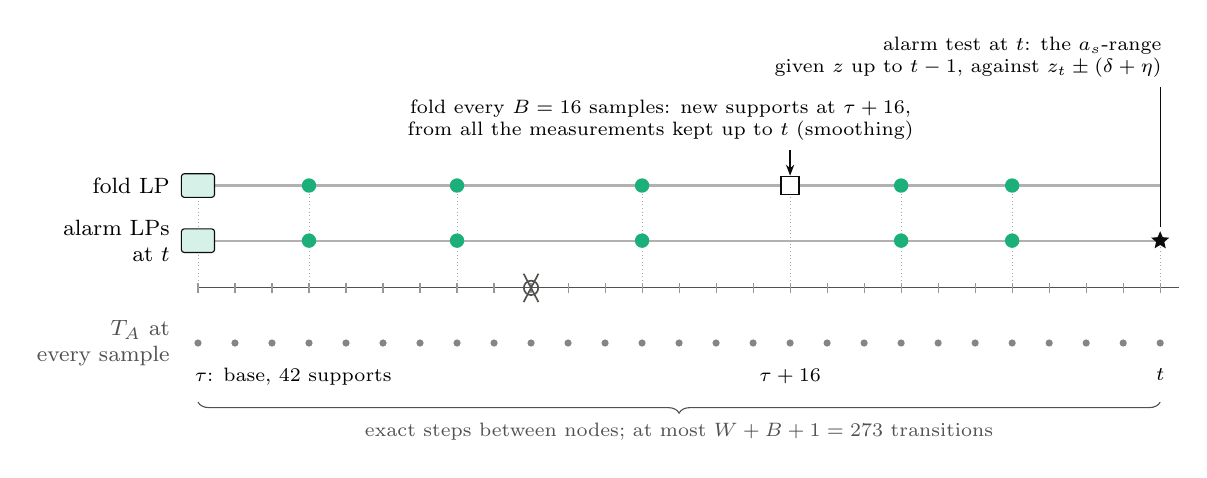
\begin{tikzpicture}[x=0.47cm, y=1cm, font=\footnotesize]
\def\yA{0.6}  % lane: the alarm LPs at t
\def\yF{1.3}  % lane: the fold LP
% sample axis and T_A at every sample
\draw[muted, line width=0.4pt] (0,0) -- (26.5,0);
\foreach \i in {0,...,26} \draw[muted!60] (\i,-0.06) -- (\i,0.06);
\foreach \i in {0,...,26} \fill[muted!70] (\i,-0.7) circle (1.3pt);
\node[anchor=east, muted, align=right] at (-0.5,-0.7) {$T_A$ at\\every sample};
% the two lanes
\foreach \y/\lab in {\yA/{alarm LPs\\at $t$}, \yF/{fold LP}} {
  \draw[muted!45, line width=0.8pt] (0,\y) -- (26,\y);
  \node[anchor=east, align=right] at (-0.5,\y) {\lab};
}
% guides from the axis to the nodes
\foreach \i in {0,3,7,12,19,22} \draw[muted!50, line width=0.3pt, densely dotted] (\i,0) -- (\i,\yF);
\draw[muted!50, line width=0.3pt, densely dotted] (16,0) -- (16,\yF);
\draw[muted!50, line width=0.3pt, densely dotted] (26,0) -- (26,\yA);
% base at tau, in both lanes
\foreach \y in {\yA,\yF} \node[draw=ink, fill=cWM!18, rounded corners=1pt, minimum width=0.42cm, minimum height=0.3cm,
  inner sep=0pt] at (0,\y) {};
% kept measurements, in both lanes
\foreach \y in {\yA,\yF} \foreach \i in {3,7,12,19,22} \fill[cWM] (\i,\y) circle (2.6pt);
% a measurement redundant at arrival: not kept, in neither lane
\draw[muted, line width=0.6pt] (9,0.0) circle (2.6pt);
\draw[muted, line width=0.6pt] (8.8,-0.18) -- (9.2,0.18) (8.8,0.18) -- (9.2,-0.18);
% the fold target, in the fold lane only
\node[draw=ink, fill=white, line width=0.6pt, minimum size=6.5pt, inner sep=0pt] (target) at (16,\yF) {};
\node[anchor=south, align=center, font=\scriptsize] (foldtxt) at (12.5,1.75)
  {fold every $B=16$ samples: new supports at $\tau+16$,\\from all the measurements kept up to $t$ (smoothing)};
\draw[-{Stealth[length=4pt]}, ink, line width=0.5pt] (16,1.75) -- (target.north);
% the current sample, in the alarm lane only
\node[star, star points=5, star point ratio=2.2, fill=ink, inner sep=1.1pt] at (26,\yA) {};
\node[anchor=south east, align=right, font=\scriptsize] at (26.3,2.55)
  {alarm test at $t$: the $a_s$-range\\given $z$ up to $t-1$, against $z_t\pm(\delta+\eta)$};
\draw[ink, line width=0.4pt] (26,\yA+0.17) -- (26,2.55);
% sample labels
\node[anchor=north west, font=\scriptsize] at (-0.35,-0.9) {$\tau$: base, 42 supports};
\node[anchor=north, font=\scriptsize] at (16,-0.9) {$\tau+16$};
\node[anchor=north, font=\scriptsize] at (26,-0.9) {$t$};
% the window length
\draw[decorate, decoration={brace, mirror, amplitude=4pt}, muted] (0,-1.45) -- (26,-1.45)
  node[midway, below=4pt, muted, font=\scriptsize] {exact steps between nodes; at most $W+B+1 = 273$ transitions};
\end{tikzpicture}

\caption{The window of WM between two folds (schematic, not to scale). The states $(a_c, a_s)$ appear at the nodes
only, and the two kinds of LP have different nodes: the alarm LPs at $t$ the base at $\tau$ (box), the kept
measurements (filled circles, at most $K_{\mathrm{cap}} = 64$) and $t$ (star); the fold LP the base, the measurements
kept up to $t$, the target $\tau+16$ (square) and a node at $t$. A measurement redundant at arrival (crossed circle) is not kept and
is a node of neither. $T_A$ appears at every sample.}
\label{fig:window}
\end{figure*}

Between nodes the steps are exact:
$x_b = M^L x_a + \sum_{k<L} M^k e_3 w_{b-1-k}$, with every $|w_j|\le\rho$ explicit. $M^L$ and $M^k e_3$ are the exact
powers of the exact model, each rounded once. The states $(a_c, a_s)$ appear at the nodes only ($\tau$, the kept
measurements and the objective sample: $t$ for the alarm, $\tau+16$ for a fold) and $T_A$ at every sample. Between nodes, $a_c$ and $a_s$ stay in the
box by convexity, so only the box rows of $T_A$ are needed. Apart from dropped measurements, the window is exact.

A measurement that the primal $a_s$-range (not
certified) shows redundant at arrival is dropped; dropping only removes a constraint, so it is sound whatever that value
is. Above $K_{\mathrm{cap}}$ kept measurements, the one inactive longest is
evicted. Both only remove constraints.

The alarm at $t$ uses the $a_s$-range of the window given $z$ up to $t-1$. WM flags only when a \emph{certified} bound
separates it from $[z_t-\delta-\eta,\ z_t+\delta+\eta]$, with $\eta = 10^{-9}$\,\degC\ and the slab rounded outward. A
primal value that points to an alarm the certificate cannot prove raises nothing; $z_t$ is then dropped.

Every $B = 16$ samples the base is folded from $\tau$ to $\tau+16$. Each of the 42 new supports is the maximum of
$d_i\cdot x_{\tau+16}$ over the window \emph{with every measurement kept up to the current
sample $t$}, raised to at least
its certified bound and then clamped. This is the smoothing rule: the new base carries what later measurements say
about the past state. The filtering rule would use the measurements up to $\tau+16$ only.

$\eta$ encloses the floating-point error of the data. The simulator computes $z$ from two binary64 simulations; an a
priori bound puts the data of every healthy run within \sci{5}{-11}\,\degC\ of data that an admissible run of the exact
model explains with $|v|\le\delta$. $\eta$ is 20 times that.
% src: FREEZE-V2.md section 1 (window LP, fold, eta and its a priori bound); FREEZE-V3.md section 1

\subsection{Certificates}\label{sec:cert}

Every alarm bound and every fold bound is a weak-duality bound computed from the solver's multipliers, with every
variable boxed, the floating-point rounding of the bound's own evaluation bounded explicitly, and the rounding of each
LP coefficient enclosed (each is its exact value rounded once). So the bound holds for the LP with exact coefficients,
whatever the solver's tolerance \citep{neumaier2004,jansson2004}. With every variable boxed it holds for \emph{any}
multiplier vector: a solver stopped early gives a looser bound, never an unsound one. The floating-point model is IEEE
binary64 with rounding to nearest and gradual underflow; a product's error beyond the relative model is at most
$2^{-1075}$, and the bound includes that term.

An audit variant evaluates every bound again in exact rational arithmetic. Over all development rows, 3,548,402 bounds
were audited with no violation; the smallest slack was \sci{8.2}{-16}\,\degC. Under simulated solver failures a further
12,572,172 bounds, 425,757 of them fallback bounds, were audited with no violation.
% src: FREEZE-V2.md section 1 "The certificate"; FREEZE-V3.md section 1 floating-point model; DIAG-3-RESULTS.md AF1
% (3,548,402, 8.2e-16) and amendment 10 R3 table (a, b 4,319,122 each, e 3,933,928; implied 39,033 + 386,724)

\begin{proposition}[soundness of WM]\label{prop:wm}
Under the model, WM never flags an admissible record and never flags before $\tstar$, and every flag carries a
certificate.
\end{proposition}
\begin{proof}[Proof sketch]
Let $\mathfrak{X}(t\mid t-1)$ be the explanations of the measurements up to $t-1$ under the exact model, as states at
$t$, with slabs $\delta+\eta$. The window LP with exact coefficients contains $\mathfrak{X}$ when its base at $\tau$
contains the projection of the explanations at $\tau$: its rows are the model's dynamics, the $a_c$ and $a_s$ boxes
hold by convexity, and the $w$ and $T_A$ boxes are the model's. The certificate bounds the ideal window, not the
solver's rounded one. The start is the template's start. Dropping and evicting only remove constraints. Each fold
support is at least the maximum over the ideal window and the clamps hold for every reachable state, so the new base
contains the explanations at $\tau+16$. An alarm needs a certified separation. The full proof is in
Appendix~\ref{app:proof}.
\end{proof}

\subsection{When the solver does not solve}\label{sec:fallback}

Every LP of WM has two outcomes: \emph{solved} (status optimal, after at most three attempts: dual simplex without
presolve, interior point without presolve, dual simplex with presolve) or \emph{failed} (any other status; an exception
of one of six types from the solver call: \texttt{RuntimeError}, \texttt{ValueError}, \texttt{IndexError},
\texttt{OverflowError}, \texttt{ZeroDivisionError} or \texttt{FloatingPointError}; or an answer that is not finite).
Any other exception stops the run without an alarm. A \texttt{RuntimeError} raised inside a fold outside the solver
call is recorded as an uncertified alarm, and any other exception there stops the run; which the scoring rules count as a soundness failure. Neither happened in validation 3. WM never uses a value from a failed LP. A solver's
``infeasible'' is one more failure, not a proof: an alarm needs a certified separation. The fallbacks are outer bounds
(Table~\ref{tab:fallback}).

\begin{table*}[t]
\centering\small
\caption{Fallbacks of WM when an LP fails.}\label{tab:fallback}
\begin{tabular}{>{\raggedright}p{0.24\linewidth}>{\raggedright}p{0.42\linewidth}>{\raggedright\arraybackslash}p{0.24\linewidth}}
\toprule
failed LP & fallback & why it is sound\\
\midrule
one side of the $a_s$-range & that side's box bound; $z_t$ not kept & the box contains every state\\
one side of the alarm certificate & that side's box bound & the same\\
one direction of a fold & the certified maximum over $P_J\cap\text{box}$, $J$ the solved faces of the same fold; if
that LP in three variables fails too, the a priori clamp & the window's states lie in $P_J\cap\text{box}$\\
every direction of a fold & reset: base $=$ the a priori clamps, no kept measurements, $\tau \mathrel{+}= B$ & the
clamps hold under the exact model\\
\bottomrule
\end{tabular}
\end{table*}

This path was added after the failure of Section~\ref{sec:val2}. Its tests are in Section~\ref{sec:inject}.
% src: FREEZE-V3.md section 1 tables

\section{Protocol}\label{sec:protocol}

All development (design, diagnosis, tuning) used seeds 430000--430099. Validation seeds 440000--440999 were reserved,
and the generator refuses them unless a freeze record is approved and its manifest matches. Each validation followed
the same order:
\begin{enumerate}
\item A freeze document fixes the hypothesis, the candidate, the scoring rules and the seed block, and a manifest pins
  every file the run uses by sha256.
\item The full pipeline is rehearsed on development seeds.
\item A commit that changes only the document's status line approves it. The runner refuses to start without that
  line, a matching manifest, a clean tree and the fixed environment.
\item The run generates the block once; the scorer applies the fixed rules in a fixed order: integrity, then soundness
  (an alarm on an admissible run, an alarm before $\tstar$, or an uncertified alarm is a FAIL), then completeness
  (undetermined fault runs at most 1\,\%), then misses and the target.
\item Nothing is rerun except after an infrastructure failure as defined in advance; the verdict is recorded as it
  came out, with a dated record.
\end{enumerate}
Every score was reproduced byte for byte on a second machine. The scores of validations 2 and 3 were also reproduced by
an independent scorer written from the rules alone, using only the Python standard library. Each block was used once. A failed candidate is not repaired on its
block: a new candidate needs a new freeze and the next unused block. The environment was CPython 3.12.13, numpy 2.5.5,
scipy 1.18.1 and HiGHS 1.12.0.
% src: FREEZE-V1/V2/V3.md; RECORD-2026-11-19 and -21 "Provenance"

\section{Results}

\subsection{Development: loss against memory}

Table~\ref{tab:dev} gives development results only (1,081 certified detection events), not a validation. Figure~\ref{fig:memory} places these monitors, and the validated ones, by the numbers they keep.

\begin{figure}[t]
\centering
% Figure: D_paired against memory. Data: figdata/fig1_*.dat (paper/figures/make_data.py, fig1).
\begin{tikzpicture}
\begin{semilogxaxis}[paperaxis,
  width=0.92\linewidth, height=6.2cm,
  xmin=1.6, xmax=170, ymin=-0.14, ymax=1.12,
  xtick={2,16,42,60,87,107}, xticklabels={2,16,42,60,87,107},
  minor xtick={}, ytick={0,0.2,0.4,0.6,0.8,1},
  xlabel={reals kept between samples (log scale)},
  ylabel={$\Dp$},
  legend style={at={(0.03,0.97)}, anchor=north west},
  legend cell align=left]
% the development curve, in memory order
\addplot[muted!55, line width=0.5pt, forget plot] table[x=mem, y=D] {figdata/fig1_dev.dat};
% development points: filled; validation points: open
\addplot[only marks, mark=*, mark size=2.4pt, cIM, forget plot]
  table[x=mem, y=D, restrict expr to domain={\thisrow{fam}}{0:0}] {figdata/fig1_dev.dat};
\addplot[only marks, mark=square*, mark size=2.2pt, cTS, forget plot]
  table[x=mem, y=D, restrict expr to domain={\thisrow{fam}}{1:1}] {figdata/fig1_dev.dat};
\addplot[only marks, mark=diamond*, mark size=2.8pt, cWM, forget plot]
  table[x=mem, y=D, restrict expr to domain={\thisrow{fam}}{2:2}] {figdata/fig1_dev.dat};
\addplot[only marks, mark=square, mark size=3.6pt, cTS, line width=0.8pt, forget plot]
  table[x=mem, y=D, restrict expr to domain={\thisrow{fam}}{1:1}] {figdata/fig1_val.dat};
\addplot[only marks, mark=diamond, mark size=4.2pt, cWM, line width=0.8pt, forget plot]
  table[x=mem, y=D, restrict expr to domain={\thisrow{fam}}{2:2}] {figdata/fig1_val.dat};
% legend entries for the two data sets (ink markers)
\addlegendimage{only marks, mark=*, mark size=2.2pt, ink}
\addlegendentry{development (1,081 events)}
\addlegendimage{only marks, mark=o, mark size=3pt, ink, line width=0.8pt}
\addlegendentry{validation (fresh blocks)}
% direct labels (layout only; values are in the data files)
\node[lab, anchor=north west] at (axis cs:2.1,-0.02) {IM (reference)};
\node[lab, anchor=north] at (axis cs:16,0.10) {inv4p};
\node[lab, anchor=west] at (axis cs:46,0.38) {TS};
\node[lab, anchor=east] at (axis cs:57,0.66) {$W=64$};
\node[lab, anchor=south east] at (axis cs:69.5,0.825) {$W=128$};
\node[lab, anchor=north west] at (axis cs:78,0.815) {$W=192$};
\node[lab, anchor=south east] at (axis cs:85,1.0) {$W=256$};
\node[lab, anchor=north west] at (axis cs:109,0.985) {WM};
\end{semilogxaxis}
\end{tikzpicture}

\caption{$\Dp$ against the reals a monitor keeps between samples. Filled markers: development (1,081 certified
events); open markers: validation (inv4p and TS on validation 1, WM on validation 3). TS's two markers coincide
(0.386 on development, 0.387 on validation 1). For a window the count is the 42
supports of its base plus the largest number of measurements it kept on that data; their sample indices, $\tau$ and
the LP workspace are not counted. IM is the reference, with $\Dp = 0$ by definition. The development points of the windows come from the
compressed window of the records (version E), which WM equals at $W = 256$ on these rows.}
\label{fig:memory}
\end{figure}

\begin{table*}[t]
\centering\small
\caption{Development: $\Dp$ against the memory of the monitor. The windows are the compressed window of the
records (version E), which WM equals on these rows at $W = 256$. ``At $\tstar$'': detections at $\tstar$. Last column: without the ten rows of
the four diagnosis runs and their control.}\label{tab:dev}
\begin{tabular}{llllll}
\toprule
monitor & state & $\Dp$ & misses & at $\tstar$ & $\Dp$ without diagnosis rows\\
\midrule
template TS only & 42 numbers & 0.386 & 4 & 897 & 0.512\\
window $W = 64$ & $\le18$ kept & 0.643 & 0 & 1037 & 0.905\\
window $W = 128$ & $\le28$ kept & 0.815 & 0 & 1063 & 0.980\\
window $W = 192$ & $\le35$ kept & 0.824 & 0 & 1073 & 0.986\\
window $W = 256$ & $\le45$ kept & 0.9992 & 0 & 1079 & 0.9987\\
\bottomrule
\end{tabular}
\end{table*}

The curve is not smooth: between $W = 192$ and 256 the gain comes from a few runs with slow drift whose separating
information lies far back. On 430010 (drift 0.0005\,\degC/s, ramp ambient), $W = 192$ detects at 3,449 and $W = 256$ at
$\tstar = 695$; its two arms give 5,508 of the 5,768 samples of paired lag that $W = 256$ gains over $W = 192$
(95.5\,\%). Figure~\ref{fig:trace} shows this run. With a cap of 64, development data never kept more than 45 measurements, so nothing was evicted. Caps of
40 and 32 detected identically on all 1,320 rows, with 420 and 21,821 evictions.
% src: DIAG-3-RESULTS.md "size-loss curve"; amendment 6 part 2 (K1, K2, K = 40 table, K = 32)
% src (figures): paper/figures/make_data.py -> figdata/figures.json; inv4p DEV D_paired 0.147 scored there

\paragraph{Smoothing against filtering.} On the four diagnosis runs, the filtering fold never recovers run 430027 at
any $W$ (it stays at 1,429 against $\tstar = 579$), and recovers 430010 only to 3,449 at $W = 256$ ($\tstar = 695$). The
smoothing fold detects both at $\tstar$ (at $W = 128$ and $W = 256$). On validation 3's block the window with the
filtering fold (B5, Section~\ref{sec:baselines}) had a paired lag of 3,782\,s against WM's 1,264\,s and missed 4
events against none.
% src: DIAG-3-RESULTS.md phase 1 tables

\begin{figure}[t]
\centering
% Figure: development run 430010 (drift 0.0005 C/s, E0, ramp). Data: figdata/fig2_trace.dat (make_data.py, fig2).
% Columns: k, z (shifted), and the a_s-range each monitor tests z_k against (lo, hi). delta = 0.3.
\begin{tikzpicture}
\begin{groupplot}[group style={group size=1 by 2, vertical sep=1.6cm},
  paperaxis, width=0.86\linewidth, unbounded coords=jump]
% (a) the upper edge of the acceptance band, hi + delta, near t*
\nextgroupplot[height=5.2cm, xmin=670, xmax=700, ymin=-0.80, ymax=-0.69, restrict x to domain=660:710,
  restrict y to domain=-1.2:-0.4, ylabel={$^\circ$C (shifted)}, xlabel={sample $k$},
  title={(a) upper edge $\bar a_s+\delta$ of the band each $z_k$ is tested against},
  legend style={at={(0.98,0.03)}, anchor=south east}, legend cell align=left]
\addplot[only marks, mark=*, mark size=1pt, muted!70] table[x=k, y=z] {figdata/fig2_trace.dat};
\addlegendentry{measurement $z_k$}
\addplot[cIM, densely dashed, line width=0.9pt] table[x=k, y=imtop] {figdata/fig2_trace.dat};
\addlegendentry{IM}
\addplot[cTS, dotted, line width=1.1pt] table[x=k, y=tstop] {figdata/fig2_trace.dat};
\addlegendentry{TS}
\addplot[cWM, line width=0.9pt] table[x=k, y=wmtop] {figdata/fig2_trace.dat};
\addlegendentry{WM}
\addplot[only marks, mark=o, mark size=3.2pt, ink, line width=0.6pt, forget plot,
  restrict expr to domain={\thisrow{k}}{695:695}] table[x=k, y=z] {figdata/fig2_trace.dat};
\node[lab, anchor=south east] at (axis cs:694.4,-0.7) {$z_{695}$: above WM's edge only};
% (b) the width of the range over the whole record, as a running median
\nextgroupplot[height=5.2cm, ymode=log, xmin=0, xmax=3600, ymin=0.02, ymax=0.3,
  ylabel={width ($^\circ$C)}, xlabel={sample $k$},
  title={(b) width of the $a_s$-range, median over 61 samples},
  ytick={0.02,0.05,0.1,0.2}, yticklabels={0.02,0.05,0.1,0.2}]
\addplot[cIM, densely dashed, line width=0.8pt] table[x=k, y=immed] {figdata/fig2_trace.dat};
\addplot[cTS, dotted, line width=1pt] table[x=k, y=tsmed] {figdata/fig2_trace.dat};
\addplot[cWM, line width=0.8pt] table[x=k, y=wmmed] {figdata/fig2_trace.dat};
\draw[muted, line width=0.4pt, dashed] (axis cs:496,0.02) -- (axis cs:496,0.3);
\draw[muted, line width=0.4pt, dashed] (axis cs:695,0.02) -- (axis cs:695,0.3);
\draw[muted, line width=0.4pt, dashed] (axis cs:3575,0.02) -- (axis cs:3575,0.3);
\node[lab, anchor=north east, align=right] at (axis cs:490,0.29) {fault\\onset 496};
\node[lab, anchor=north west, align=left] at (axis cs:700,0.29) {WM flags\\at $t^\ast=695$};
\node[lab, anchor=north east, align=right] at (axis cs:3565,0.29) {IM and TS\\flag at 3575};
\node[lab, anchor=south] at (axis cs:2300,0.125) {IM (dashed), TS (dotted)};
\node[lab, anchor=north] at (axis cs:130,0.029) {WM};
\end{groupplot}
\end{tikzpicture}

\caption{Development run 430010 (drift 0.0005\,\degC/s from sample 496, E0, ramp ambient; $\tstar = 695$).
(a)~The upper edge of the band each measurement is tested against, $\bar a_s+\delta$, with $\bar a_s$ the top of the
monitor's $a_s$-range given the past; for IM and TS a measurement above the edge is an alarm. For WM the edge drawn is
the primal value of its range LP; its alarm uses the certified bound and the slab $\delta+\eta$, with a certified
margin of $-0.29$\,m\degC\ at sample 695. There the measurement lies 0.3\,m\degC\ above WM's edge and about
5\,m\degC\ below the edges of IM and TS. (b)~The width of the $a_s$-range as a median over 61 samples centred on each
sample, so each curve stops 30 samples before its last sample.}
\label{fig:trace}
\end{figure}

\subsection{Validation 1: the template tier}\label{sec:val1}

Block 440000--440199 (9,600 runs; 7,201 certified events, 4 undetermined fault runs).

\begin{table*}[t]
\centering\small
\caption{Validation 1. Seed bootstrap; misses of IM on this block: 24.}\label{tab:val1}
\begin{tabular}{lllllll}
\toprule
 & target & $\Dp$ & bootstrap 95\,\% & misses & later than IM & verdict\\
\midrule
inv4p (16 numbers) & 0.10 & 0.152 & $[0.107, 0.205]$ & 20 & 0 & PASS\\
TS / cyl16p (42 numbers) & 0.25 & 0.387 & $[0.323, 0.452]$ & 16 & 0 & PASS\\
\bottomrule
\end{tabular}
\end{table*}

Neither monitor had a soundness finding: no alarm on any of the 2,395 admissible runs. The C float64 builds equal the
Python implementation on all 9,600 runs.
% src: RECORD-2026-11-18-validation.md Verdicts

\subsection{Validation 2: the window tier fails on one LP}\label{sec:val2}

Block 440200--440399. The window (then without the fallback path of Section~\ref{sec:fallback}) reached $\Dp = 0.995$
with no miss (IM missed 14). On one healthy run with edge noise (440243, E0, ramp), one fold LP ended unsolved in HiGHS
in all three attempts at $t = 945$, and the frozen code recorded an uncertified alarm. Under the frozen order, that row
is a soundness violation and an uncertified alarm, and the verdict is \textbf{FAIL} before any accuracy rule is
reached. The accuracy numbers are reported with the failure and are not a validation.

A diagnosis afterwards, outside the scored run, replayed the row deterministically. The failure was confined to one of
the 42 fold directions; the other 41 solved faces bound that direction at $-0.209$\,\degC\ (its previous base bound
was $-0.187$ and its a priori bound 1.683). That observation became the fallback of Section~\ref{sec:fallback}.
% src: RECORD-2026-11-19-validation.md (verdict, diagnosis)

\subsection{Validation 3: the window tier with its fallback path}\label{sec:val3}

Block 440400--440599.

\begin{table*}[t]
\centering\small
\caption{Validation 3: WM with $W = 256$, $B = 16$, $K_{\mathrm{cap}} = 64$. Seed bootstrap; misses of IM on this
block: 27.}\label{tab:val3}
\begin{tabular}{lllllll}
\toprule
 & target & $\Dp$ & bootstrap 95\,\% & misses & uncertified & verdict\\
\midrule
WM / F3 & 0.80 & 0.9952 & $[0.9899, 0.9995]$ & 0 & 0 & PASS\\
\bottomrule
\end{tabular}
\end{table*}

Figure~\ref{fig:cells} shows where the lag of each monitor lies.

\begin{figure*}[t]
\centering
% Figure: validation 3, lag per fault cell, IM against WM. Data: figdata/fig4_cells.dat (make_data.py, fig4).
% Rows (i): jump 0.5, jump 0.2, stuck, noise x2, gain 0.01, drift 0.02, 0.005, 0.002, 0.001, 0.0005 (C/s).
\begin{tikzpicture}
\begin{semilogxaxis}[paperaxis,
  width=0.62\linewidth, height=7.2cm,
  xmin=0.5, xmax=1e6, ymin=-0.6, ymax=9.6, y dir=reverse,
  ytick={0,...,9},
  yticklabels={jump 0.5\,$^\circ$C, jump 0.2\,$^\circ$C, stuck, noise $\times2$, gain 1\,\%, drift 0.02, drift 0.005,
               drift 0.002, drift 0.001, drift 0.0005},
  xtick={1,10,100,1000,10000,100000,1000000},
  xlabel={lag summed over the cell's certified events (s; misses count $N-t^\ast$)},
  ymajorgrids=true, xmajorgrids=true,
  legend style={at={(0.08,0.03)}, anchor=south west}, legend cell align=left]
\addplot[only marks, mark=*, mark size=2.4pt, cIM] table[x=im, y=i] {figdata/fig4_cells.dat};
\addlegendentry{IM}
\addplot[only marks, mark=diamond*, mark size=3pt, cWM,
  restrict expr to domain={\thisrow{wm}}{1:1e9}] table[x=wm, y=i] {figdata/fig4_cells.dat};
\addlegendentry{WM}
% WM's lag is 0 in seven cells: open diamonds at the left edge
\addplot[only marks, mark=diamond, mark size=3pt, cWM, line width=0.7pt,
  restrict expr to domain={\thisrow{wm}}{-1:0.5}] table[x expr=0.7, y=i] {figdata/fig4_cells.dat};
\addlegendentry{WM, lag 0 (left edge)}
% IM's misses (selective labels)
\node[lab, anchor=west] at (axis cs:40000,1) {8 missed};
\node[lab, anchor=west] at (axis cs:75000,8) {2 missed};
\node[lab, anchor=west] at (axis cs:125000,9) {17 missed};
\end{semilogxaxis}
\end{tikzpicture}

\caption{Validation 3: the lag of IM and WM in each fault cell, summed over the cell's certified events, with a miss
counted as $N-\tstar$ (log scale). Drift rates in \degC/s. WM's lag is 0 in seven cells (open diamonds at the left
edge). IM's 27 misses are in the three labelled cells.}
\label{fig:cells}
\end{figure*}

\begin{itemize}
\item Of the 8,000 fault runs, 7,255 are certified events, 742 are certified consistent (the fault never contradicts
  the model within the record, so the run is admissible) and 3 are undetermined. Of the 742, 400 are the stuck sensor
  under E0: with a constant command the frozen reading, which the simulator keeps adding fresh noise to, stays
  explainable. The other 342 are drifts of 0.0005 and 0.001\,\degC/s; under E1 every stuck run is an event. Neither IM nor WM alarmed on any of
  the 2,342 admissible runs: the 1,600 healthy runs and these 742.
% src: RECORD-2026-11-21-validation.md lines 84-92
\item No soundness finding. 7,255 certified events; 7,243 detected exactly at $\tstar$ (IM: 5,257). Lag p90 0\,s and
  maximum 212\,s (IM: 55\,s and 2,215\,s; the scorer's percentile is the order statistic at the nearest index). No run
  was later than IM.
\item 7,258 alarms, each recorded with its certificate flag and a finite negative certified margin, the signed
  distance from WM's certified bounds on $a_s$ to the slab of radius $\delta+\eta$ around the measurement, rounded
  outward (the largest $-0.0147$\,m\degC); three of them on fault runs the oracle left undetermined. The LP data
  behind the certificates are not archived.
\item On all 7,997 certified fault runs the oracle's own bounds leave room on both sides of $\delta$: at least
  \sci{1.07}{-7}\,\degC\ on the inconsistent side at $\tstar$ (the 7,255 events), at least \sci{2.90}{-6}\,\degC\ on
  the consistent side before $\tstar$, and at least \sci{5.15}{-4}\,\degC\ on the 742 certified-consistent runs, more
  than $2\times10^5$ times the model gap of Corollary~\ref{cor:wm}. The certificates are sound
  (Lemmas~\ref{lem:ocert} and~\ref{lem:olow}) and the shift by 25\,\degC\ is exact on these prefixes, so the
  oracle's certified $\tstar$ on this block is the exact model's, and the 742 certified-consistent fault runs are
  consistent under the exact model.
% src (room): RECORD-2026-11-23-oracle-margin.md (plan ORACLE-MARGIN-PLAN.md, e2772d92); 742 runs' room from its
% margins.jsonl (RECORD-2026-11-23-review3-checks.md)
\item The remaining lag sits in three cells: drift 0.0005 and 0.001\,\degC/s with ramp ambient, and drift
  0.002\,\degC/s with rw ambient. Drifts carry 99.8\,\% of IM's paired lag; over all certified events with
  a miss counted as $N-\tstar$, as in Figure~\ref{fig:cells}, 91.8\,\%.
\item WM detected 12 events after $\tstar$, all in slow drift cells. At each of them the oracle's lower bound on $d^\ast$
  at $\tstar$ exceeds $\delta$ by at least \sci{1.07}{-7}\,\degC, more than 100 times $\eta$ plus the model gap of
  Corollary~\ref{cor:wm}. So with WM's own semantics, its slab $\delta+\eta$ and its matrix, the full history is
  already inconsistent at $\tstar$, and these delays are losses of its compressed state. Whether $\eta$ changes which
  measurements the window keeps or its fold bounds, and so where it loses, was not isolated.
\item The fallback path never ran on this block. WM solved 53,968,652 LPs with 722 retries (on 320 runs), and every LP was solved
  within its three attempts. The validation supports the window's accuracy and the soundness of its normal path; the
  fallback path rests on its proof and on Section~\ref{sec:inject}.
\item At most 65 measurements kept, at most 445 LP rows and 679 variables.
\end{itemize}
% src: RECORD-2026-11-21-validation.md
% src (12 late events): RECORD-2026-11-22-review-checks.md, diag/eta_check.py (1.06e-7 on the Mac with other
% multipliers; both are lower bounds); 1.07e-7 = RECORD-2026-11-23-oracle-margin.md, which covers these 12

\paragraph{Other metrics.} $\Dp$ weighs large lags heavily: on validation 3 the three slowest drift cells carry
97.9\,\% of IM's paired lag. Table~\ref{tab:metrics} scores the validated monitors over all certified events, with
every lag capped at 30\,s, and by percentiles of the lag; the order of the monitors is the same under each. The
targets of the hypotheses (0.10, 0.25 and 0.80) were fixed for the point estimate of $\Dp$; the bootstrap intervals are
descriptive and are not part of the decision rule.

\begin{table*}[t]
\centering\small
\caption{The validated monitors under other metrics. ``All events'': the ratio $1-L_m/L_{\mathrm{IM}}$ over every
certified event, a miss counted as $N-\tstar$; ``capped'': the same with every lag capped at 30\,s. Percentiles over
the detected events, with linear interpolation (the scorer of Section~\ref{sec:val3} takes the nearest index;
for IM's p90 both give 55\,s).}\label{tab:metrics}
\begin{tabular}{llllll}
\toprule
monitor (block) & $\Dp$ & all events & capped & lag p90 / p99 (s) & misses / events\\
\midrule
IM (validation 1) & 0 & 0 & 0 & 53 / 808 & 24 / 7,201\\
inv4p (validation 1) & 0.152 & 0.132 & 0.263 & 38 / 749 & 20 / 7,201\\
TS (validation 1) & 0.387 & 0.368 & 0.389 & 21 / 527 & 16 / 7,201\\
IM (validation 3) & 0 & 0 & 0 & 55 / 833 & 27 / 7,255\\
WM (validation 3) & 0.9952 & 0.9960 & 0.9929 & 0 / 0 & 0 / 7,255\\
\bottomrule
\end{tabular}
\end{table*}
% src: diag/metric_sensitivity.py on the recorded rows (RECORD-2026-11-22-review-checks.md)

\subsection{The fallback path under injected solver failures}\label{sec:inject}

A separate preregistered test injected solver failures into WM on 1,200 fresh runs (25 seeds of a separate namespace)
in six settings: 1\,\% and 10\,\% of the LPs of fold directions; 1\,\% of the $a_s$-range and certificate LPs; every
direction of every fourth fold; 10\,\% of fold directions together with every $P_J$ LP; every upper certificate LP.
All criteria held in every setting: no alarm on an admissible run, none before $\tstar$, every alarm certified, at most
65 kept measurements, the fallback counters equal to the injection log, and every fallback path reached (for example
375,725 implied $P_J$ bounds and 22,600 full resets). The exact audit of two settings checked 7,300,179 bounds with no
violation.

The cost was in detection. With 1\,\% and 10\,\% fold failures nothing was missed; one detection in the 10\,\% setting
came 45 samples later than without injection. With 1\,\% of the $a_s$-range and certificate LPs failing, 22 detections
came later (median 6 samples), nothing was missed and $\Dp$ was 0.977; 14 events that IM detects were detected after
IM. With every fourth fold reset, 30 events were missed and $\Dp$ was $-5.21$; with every upper certificate failing,
174 were missed and $\Dp$ was $-29.24$. In these two settings WM was later than IM, or missed, on 232 and 752 of the
events that IM detects.
% src: RECORD-2026-11-21-fb.md (settings table: later, missed, D_paired, later than v2 or missed where v2 detects);
% settings = FB-PLAN.md table

\paragraph{The solver's process.} In the runs above the LPs run in WM's own process. A solver that ends its process (as
the interior-point solver did in 8 of the oracle's 117,606 attempts in validation 3, by a segmentation fault) would end
the run before any fallback could see it. In a variant, WM's LPs run in a child process that persists across LPs; if
the child ends or does not answer in 120\,s, it is replaced and the attempt counts as failed, so the fallbacks of
Section~\ref{sec:fallback} apply. Without injection the variant equals WM in every recorded field but time on 6 development
rows. On the 1,400 development rows the child then ended itself before 15,320 LPs, in all three attempts of each (half
by exit, half by a segmentation fault; two per thousand fold LPs, one per thousand $a_s$-range LPs, a fifth of the LPs
of implied bounds and half of the certificate LPs). Every run completed. No alarm came on an admissible run or before
$\tstar$, every alarm was certified, the fallback counters equalled the injection log on every row, and at most 65
measurements were kept. Again the cost was in detection: 497 detections came later (median 5 samples) and 3 events
with slow drift were missed; none came earlier. Two documented paths lead there: an alarm whose certificate cannot be
computed is not raised, and a measurement checked against a failed $a_s$-range LP is not kept. Their shares were not
computed.
% src: RECORD-2026-11-21-iso.md; ISOLATION-PLAN.md section 2 (rates); RECORD-2026-11-21-validation.md lines 193-200
% (8 of 117,606 oracle attempts, all highs-ipm)

\subsection{Precision and microcontrollers}\label{sec:mcu}

A build is named by the precision of its tables and supports; in every build the command part $S$ is binary64, on
the AVR in software (faithful, not correctly rounded).
% src: MCU-NOTES.md lines 89, 109, 118

\paragraph{float32 builds.} Built with float32 tables, the template state was sound on the first validation block,
including the 800 healthy runs with noise exactly at $\pm\delta$. But TS in float32 reached $\Dp = 0.212$ (target 0.25)
and was later than IM on 52 runs; inv4p in float32 reached 0.004 with 28 misses and was later than IM on 130 runs.
Theorem~\ref{thm:dom} holds in exact arithmetic, not in float32. Neither float32 build was the object of a hypothesis.
% src: RECORD-2026-11-18-validation.md lines 92-105

\paragraph{ESP32 with float64 tables.} The frozen C implementation of TS with the validated float64 tables ran on an ESP32
(240\,MHz) on all 1,400 development rows, 5,040,000 samples. On every sample the alarm flag and a 16-byte hash of the
full state equalled the PC build's (preregistered; negative controls detected a change of $10^{-6}$ in one input and a
single flipped bit). Per sample, on the 322 rows that never flag (after a flag the state stops): 3.63\,ms median,
4.56\,ms maximum. On four earlier rows a float32 build took 0.49\,ms median against 3.72 to 3.74\,ms for float64.
% src: MCU-NOTES 2d, 2e

\paragraph{8-bit AVR with float32 tables.} On an ATmega328P (16\,MHz, 2\,KB SRAM) the float32 build used at most 602
bytes of SRAM and 28,064 bytes of flash, at 74 to 76\,ms per sample. On 30 preregistered development rows its first
flagged sample equalled the PC float32 build's on every row. Its state is not equal bit for bit: the board's binary64
is faithful but not correctly rounded, and the largest measured difference in a support was \sci{7.2}{-7}\,\degC. That
is far below the margins at which the test changes its answer, but the pads do not cover it by construction.
% src: MCU-NOTES 2c, 2f

\paragraph{The C state against the exact model.} A check in exact rational arithmetic found two gaps in the frozen C
state. (i) The command part $S$ is computed in binary64 and no pad covers its rounding: the frozen C state is sound
against the exact model for $|v|\le\delta-\varepsilon$, with $\varepsilon = \sci{4.86}{-13}$\,\degC\
(\sci{9.95}{-13}\,\degC\ on the AVR). (ii) Two start supports were \sci{1.11}{-16}\,\degC\ short; the first step absorbs
the shortfall. A revised C state closes both by construction, with the slab $\delta+\eta$ and exact start sums, so that
it is sound for $|v|\le\delta$. Preregistered checks accepted it: the same first flag as the frozen C state on all
1,400 development rows, equality bit for bit with its PC build on the ESP32 over 5,040,000 samples, and the same first
flag as its PC build on the AVR on 30 rows. On development data the fix cost no detection. It is not validated on
fresh seeds. A check planned before its run put its PC build beside the frozen C state's on all 19,200 runs of
validations 1 and 3: the same first flagged sample on every run, never earlier, and no alarm on an admissible run; on
validation 1 the frozen build reproduced the validation's recorded C detections, which equal the Python template's.
Both blocks were seen before the revised state existed, so this shows that its PC build reproduces the template's
recorded scores on validations 1 and 3, not that it is validated.
% src: C1-USED-BLOCKS-PLAN.md (8d16cca3); RECORD-2026-11-24-c1-used-blocks.md; results/v3/c-state/c1-used-blocks-8d16cca3/
The validated Python template has the same $S$ recursion and the same $\varepsilon$; a record with noise
within $\varepsilon$ of the bound makes it flag (Section~\ref{sec:wrong}). Its two rate pads are also open, at
\sci{2.1}{-21}\,\degC.
% src: MCU-NOTES 2g, 2h; C1-PLAN.md

\paragraph{Several sensors.} The tables depend on the model, the template and the assumptions, not on the data, and
the C state of one sensor is one structure, so sensors with the same model and assumptions share one set of tables: 37,036 bytes in
float64, with 360 bytes of state per sensor (the 42 supports, the command part, the flag and the sample counter). Each
added sensor adds its state and its step, 3.63\,ms median on the ESP32; no run had more than one sensor on a board.
Soundness holds record by record: if every sensor's record meets the assumptions, a sound monitor flags none of them,
however many there are (for the frozen implementations of TS, within the restrictions of the previous paragraph). A
detector tuned to a false-alarm probability $\alpha$ per sensor over a record flags at least one of $N$ independent
healthy sensors with probability
$1-(1-\alpha)^N$, 0.049 for $\alpha = 0.01$ and $N = 5$, unless its threshold is raised, which delays detection. For a
bank of set-membership monitors, what grows with $N$ is the chance that the assumptions fail on some sensor, a question
about the model rather than about a threshold.
% src: experiments/v3/c/v3_state.h; sizeof on the PC build (clang, arm64), 2026-11-23: the arrays of
% frozen/c/tables_cyl16p_double.h 37,036 bytes, v3_state 360 bytes (float build: 20,540 and 192; 189 on the AVR with
% -mdouble=64); the same on the ESP32 (xtensa-esp32-elf-gcc static asserts, review r7); 3.63 ms = MCU-NOTES 2e

\subsection{Baselines}\label{sec:baselines}

The comparison was planned, and its configurations frozen, before it ran (approval commit \texttt{9438dffa}). It runs
on the block of validation 3, whose results for WM and IM were already known, so it is a fixed comparison on a used
block and not a new validation. Five families get the same prior as ours, the box of $T_A$ and the boxes of $a_c$ and
$a_s$ it implies, at every sample, and B1 to B3, as a tuning option, the bounds of Lemma~\ref{lem:err} in four
directions of the error plane: B1 constrained zonotopes \citep{scott2016}; B2 zonotopes with strip intersection
\citep{alamo2005}; B3 a zonotopic observer with constant gain \citep{combastel2015}; B4 an interval observer in
cooperative form; B5 WM with the smoothing fold turned off, a forward window in the style of \citet{kesavan2001}. All
five are our implementations, and a result for one holds for its reduction and rescaling choices, not for its family
as a whole. B1
to B4 run in plain binary64 as published, without outward rounding; an alarm they raise on an admissible run or
before $\tstar$ would be reported as a soundness finding of that implementation. Each family was tuned on development
rows: at each memory budget, the configuration with the smallest paired lag among those with no such alarm.
% src: BASELINE-PLAN.md section 2 (box or box+err for B1-B3; B4 the boxes only); diag/baselines.py ERR_DIRS

\paragraph{Memory.} A monitor's memory is the number of reals it stores between samples, tables and code excluded:
TS 42 supports; WM the 42 supports of its base and at most 65 measurements, 107 in all (their sample indices are not
counted); B1 and B1s the centre, generators and constraints of their set; B2 and B3 the centre and generators; B4 and
B4s six bounds. The workspace of an LP within a sample is not counted for any method; for the methods that solve LPs
(B1, B1s, B5 and WM) the largest LP is given. The budget M1 is about 42 reals, TS's. The plan named WM's memory as the budget M2, but the
tuning set no upper limit there, and the configuration it chose for B1 stores 203 reals, nearly twice WM's 107; in the
second comparison below, B1s at M2 stores 5,963. In stored reals the comparison at M2 therefore favours B1 and B1s; it
says nothing about bytes, time or the workspace of an LP.

\paragraph{Hypotheses.} Fixed before the run, each judged by a seed bootstrap (2,000 draws over the 200 seeds) of the
difference of paired lags, ours minus the baseline's: \emph{supported} if its 95\,\% interval lies below 0,
\emph{refuted} if it lies above 0, \emph{not resolved} otherwise. H-B1: at M1, TS's paired lag is below that of each
of B1 to B4. H-B2: WM's paired lag is below B5's. H-B3: at M2, WM's paired lag is below B1's. On development rows
every configuration of every family was behind IM; the nearest, B1 at 203 reals, had 2.1 times IM's paired lag.
% src: BASELINE-PLAN.md sections 3, 4, 6 and 9 (approved 9438dffa); RECORD-2026-11-21-baselines-dev.md (DEV, the M2 note)

\paragraph{Results.} Table~\ref{tab:baselines}. The block has 7,255 certified events; IM detects 7,228 of them, with a
paired lag of 262,482\,s. All three hypotheses were supported. At M1, TS's paired lag was below that of each of B1 to
B4, by 1.9 to 12.4 million seconds over the block, and the nearest of them, B1 at 32 reals, had 7.6 times IM's paired
lag. At M2, WM's paired lag was 474,074\,s below B1's (95\,\% interval $[-517{,}380, -431{,}128]$). The closest
comparison was H-B2: the filtering window B5 lost 2,518\,s more than WM, interval $[-5{,}378, -414]$; the smoothing
fold removes two thirds of B5's paired lag, and the forward window alone already reaches $\Dp = 0.986$. The two
windows flag at the same sample on 7,237 of the 7,255 events; WM is earlier on 18, in 7 of the 200 seeds, and never
later, and it costs 34.5\,ms per sample against B5's 20.4. No method raised
an alarm on an admissible run or before $\tstar$. B1 to B4 run in plain binary64, so for them this is an observation on
these runs, not a guarantee. B1 at 203 reals had one failed LP, after which it falls back to the unconstrained hull. B1's interval rescaling
treats coefficients below $10^{-12}$ as zero, which can lose the outer property in constructed cases. B5's
7,254 alarms were all certified. A second scorer, written from the plan alone with its own random seed and percentile
rule and fixed before the block's rows existed, reproduced every number of Table~\ref{tab:baselines} and gave the
same three verdicts at 2,000 and at 20,000 draws (H-B2: $[-5{,}346, -410]$ and $[-5{,}350, -402]$).

\begin{table*}[t]
\centering\small
\caption{The two frozen comparisons on validation 3's block. Memory: reals stored between samples. Largest LP: rows
$\times$ variables; for B1 and B1s the bound of their code, $n_c+7$ equality rows and $3o+n_c+8$ generators (the decision LP comes
after one new generator and up to seven prior strips), which development data reach; B5's sizes were not recorded. Time: wall time per processed sample of one worker, 14 workers on
8 cores; it compares the methods with each other, not with a dedicated core. WM's and IM's rows are validation 3's;
TS's, B1's and B4's are the first comparison's, scored again with the second.}
\label{tab:baselines}
\begin{tabular}{lrlrrrr}
\toprule
monitor & memory & largest LP & $\Dp$ & misses & at $\tstar$ & ms/sample\\
\midrule
WM & 107 & $445\times679$ & 0.995 & 0 & 7,243 & 34.5\\
B5, filtering window & 107 & & 0.986 & 4 & 7,227 & 20.4\\
TS & 42 & none & 0.442 & 11 & 5,967 & 0.06\\
IM & 2 & none & 0 & 27 & 5,257 & \\
B1, constrained zonotope & 203 & $\le11\times36$ & $-0.81$ & 52 & 5,030 & 2.9\\
B1, constrained zonotope & 32 & $\le8\times15$ & $-6.63$ & 300 & 3,521 & 2.9\\
B4, interval observer & 6 & none & $-27.6$ & 1,799 & 790 & 0.01\\
B3, zonotopic observer & 21 & none & $-37.0$ & 2,463 & 204 & 0.08\\
B2, strip zonotope & 21 & none & $-46.8$ & 3,293 & 22 & 0.08\\
\midrule
\multicolumn{7}{l}{\emph{second comparison}}\\
B4s, interval observer & 6 & none & 0.088 & 21 & 5,593 & 0.28\\
B1s, constrained zonotope & 5,963 & $\le71\times96$ & $-2.39$ & 120 & 4,201 & 11.5\\
B1s, constrained zonotope & 32 & $\le8\times15$ & $-9.64$ & 484 & 2,848 & 3.2\\
\bottomrule
\end{tabular}
\end{table*}
% src: RECORD-2026-11-22-baselines-block.md; results/v3/baselines/block-9438dffa/scores.json; WM ms/sample = sum of
% F3 seconds / processed samples on validation 3's rows; B1 LP bound from baselines_cz.py (predict, then range(P2));
% observed (5x12, 8x33) on 440400 jump_0.5 and (8x15, 11x36) on DEV (internal review, RECORD-2026-11-22-review2.md)
% second comparison: RECORD-2026-11-23-baselines2.md; results/v3/baselines2/block-606d91cb/scores.json; B1s LP bound
% reached on DEV 430000-430001 healthy and drift_0.0005 E0 rw (71x96 and 8x15; Mac, 2026-11-24, scratch diagnostic)

\paragraph{A second comparison.} Reviews of our baseline code after the first comparison found two problems. B4 never
intersects its range with the measurement, which IM does, so IM used information B4 did not. B1's discrete choices
(exact elimination, near-ties in its reduction, prior strips) switch on the last bits of the data: on development run
430010 (drift 0.002\,\degC/s, E0, rw) a shift of the data by $10^{-15}$\,\degC\ moves its first detection among
samples 635, 1,101, 2,247 and 2,258, and the first comparison's own records of that run differ between two machines.
The first comparison stands as it ran. A second one, planned and frozen in the same way (commit \texttt{606d91cb}),
adds two versions. B4s is B4 with the measurement slab, the bounds of Lemma~\ref{lem:err} propagated by intervals, and
IM's rate rule. With IM's slab it could not be later than IM in exact arithmetic; like every baseline it uses
$\delta+\eta$ where IM uses $\delta$, so that it was never later on the block is an observation, not a guarantee. B1s is B1 with stable discrete choices and an interval
rescaling that is outer in binary64; its other steps are B1's, in plain binary64. Both were tuned on the same
development rows by the same rule, M1 again at most 42 reals and M2 again without an upper limit (B1s: $(n_c, o)$ from
$(1, 2)$ to $(64, 8)$, fifo or greedy, prior with the error bounds; B4s: $L = 0$ and B4's chosen gain), after checks
that no configuration flags an admissible development row or before $\tstar$ and that B4s is never later than IM.
The tuning chose B1s with $n_c = 1$, $o = 2$ at M1 (32 reals), B1s with $n_c = 64$, $o = 8$ at M2 (5,963 reals), and
B4s with $L = 0$ at both (6 reals). On 100 development rows with the data shifted by 0, $\pm10^{-15}$ and
$2\cdot10^{-15}$\,\degC, B1 at M2 changed its detection on 24 and no B1s configuration on more than one. The plan went
through three versions before the frozen one; one was stopped after 393 development rows, when B1s's first
rescaling, which was not outer, flagged 7 admissible rows. Hypotheses, judged as before: H-S1, WM's paired lag is
below B1s's at M2; H-S2, at M1 TS's paired lag is below B1s's (a) and below B4s's (b).
% src: BASELINE2-PLAN.md sections 0, 1, 3, 4, 7, 8 and its status block (DEV, unit and stability results)

\paragraph{Results of the second comparison.} Table~\ref{tab:baselines}, lower part. All three hypotheses were
supported. WM's paired lag was 889,162\,s below B1s's at M2 (95\,\% interval $[-981{,}119, -805{,}505]$); TS's was
2,645,818\,s below B1s's at M1 and 92,984\,s below B4s's ($[-116{,}210, -73{,}654]$). B4s was never later than IM and
was earlier on 506 of the 7,255 events, which the bounds of Lemma~\ref{lem:err} allow: IM does not use them. It
removed 8.8\,\% of IM's paired lag; TS removed 44.2\,\%. B1s was later than B1 at both budgets. In B1's own
configuration at M1 it was later on 1,765 events and earlier on 147; at M2, with 5,963 reals against B1's 203, later on
1,879 and earlier on 283. A $2\times2$ factorial on the 100 development rows of the stability check, at $(1,2)$ and
$(4,8)$, finds most of the same-configuration gap in two changes that govern the elimination of slack generators:
B1s counts an elimination as exact when its excess is at most $10^{-12}$ (B1: 0), and its interval rescaling has an
outward pad. With the tolerance at 0 alone, B1s's instability returns (4 and 27 rows of 100 move under the shifts;
B1: 16 and 24); at $(1,2)$ its paired lag is then B1's (33,051\,s against 33,445; B1s 38,806), at $(4,8)$ 25,128\,s
against 12,423 and 30,299, and with the pad off as well 17,503\,s, 72\,\% of the gap closed. B1's extra detections
and its instability come from the same last-bit decisions. The factorial does not cover B1s at $(64,8)$ or the
block. B1s at M2 had 34 failed LPs
in 28.1 million, after which it uses the unconstrained hull, as B1 does. No configuration of either comparison raised
an alarm on an admissible run or before $\tstar$; B1s and B4s run in binary64 without a proof, so for them, too, this
is an observation. The second plan was written after the first comparison's results were known and runs on the same
block: it is a second look at the same data, not a new test.
% src: RECORD-2026-11-23-baselines2.md (scores, hypotheses, B4s against IM, B1s against B1, LP failures; the
% factorial: results/v3/baselines2/b1s-factorial-f5f690eb/summary.json, DEV rows, diag/b1s_factorial.py)

\subsection{How much the results lean on the ambient box}\label{sec:ambient}

Two descriptive studies on development seeds, each fixed before its run and without pass or fail, asked how the
results depend on the assumed box and what happens when the assumptions break.

\paragraph{A wider assumed box.} On the 1,320 development rows (true ambient within $[23, 27]$) the box assumed by the
oracle and by every monitor was widened to $[22, 28]$ and $[21, 29]$, with $\tstar$ computed again for each box
(Table~\ref{tab:widebox}). Against the $\tstar$ of the frozen box, widening multiplied IM's lag by 2.9 and 3.5 and
TS's by 4.1 and 5.2, and misses rose from 8 to 32 and 55 (IM) and from 4 to 28 and 51 (TS). Most of this is not lost
by the monitors. The exact detector itself is weaker with a wider box: of the 1,081 events certified at the frozen box
it no longer detects 26 and 49 within the record and detects 55 and 32 later, all in drift cells, and it is never
earlier. Scored against the frozen $\tstar$, with a miss counted as $N-\tstar$, that costs 78,477\,s and 106,732\,s.
Against the oracle of their own box the monitors lose little more than at the frozen box: IM's lag goes from
44,363\,s to 48,129\,s and 47,991\,s, TS's from 26,680\,s to 30,518\,s and 30,786\,s, and WM's stays at 26\,s, on the
same two runs. A monitor's lag against the frozen $\tstar$ is the sum of the two, so 62 to 69\,\% of IM's and 72 to
78\,\% of TS's is the assumption's own cost, and with a wider box WM's own lag stays at the same 26\,s. TS's $\Dp$ falls from 0.386 to 0.345 and 0.334, because IM's own lag grows while the paired gap between them stays
between 12,200 and 12,700\,s. WM with a wider box is a development variant: its clamps were rebuilt for each box and
pass the vertex check of Lemma~\ref{lem:clamp} at both, and all its alarms were certified. No monitor flagged an
admissible row or flagged before the $\tstar$ of its box.
% src: RECORD-2026-11-22-widebox.md; results/v3/widebox-a196fd68/ (summary.json, split.json, check.json);
% RECORD-2026-11-21-ambient.md part (b) for the lags against the frozen t*

\begin{table*}[t]
\centering\small
\caption{The assumed box widened on the 1,320 development rows (true ambient within $[23, 27]$). Events: certified by
the oracle of that box. New: certified at that box but undetermined at the frozen box (one run, 430003, drift
0.001\,\degC/s, E1, rw); it is outside the split, and IM detects it 50\,s after its $\tstar$. Lost, later: of the 1,081
events of the frozen box, those the oracle of the wider box no longer detects within the record, or detects later. Oracle's delay: that oracle scored against the frozen $\tstar$. IM, TS,
WM: lag against the oracle of the same box, over the 1,081 events. Lags in seconds, a miss counted as $N-\tstar$; a
monitor's lag against the frozen $\tstar$ is the oracle's delay plus its own.}
\label{tab:widebox}
\begin{tabular}{lrrrrrrrr}
\toprule
box & events & new & lost & later & oracle's delay & IM & TS & WM\\
\midrule
$[23, 27]$ & 1,081 & & & & 0 & 44,363 & 26,680 & 26\\
$[22, 28]$ & 1,056 & 1 & 26 & 55 & 78,477 & 48,129 & 30,518 & 26\\
$[21, 29]$ & 1,032 & 0 & 49 & 32 & 106,732 & 47,991 & 30,786 & 26\\
\bottomrule
\end{tabular}
\end{table*}

\paragraph{Broken assumptions, healthy sensor.} With the frozen assumptions and healthy sensors, an ambient rate twice
the bound caused no alarm in any monitor on 60 runs. A rate five times the bound caused certified alarms of WM on 4 of
60 runs (two paths, both arms) and none of IM or TS; WM keeps the most information of the three and was the only one to
prove these violations. A 1\,\degC\ step in the ambient was flagged by all three on every run, 1 to 10 samples after the
step. An ambient path starting outside the box was flagged by all three within 3 samples of the start; a slow excursion
out of the box was not tested. The sensor was healthy in every run of this part, so each of these alarms reports a
broken assumption.
% src: RECORD-2026-11-21-ambient.md; results/v3/ambient/amb-443d8b30-mac/ (summary.json, report.json)

Development data had already shown why detection of slow drift depends on the box. In those cells the alarm often
comes when $z$ exceeds the top of the box plus $\delta$, so that every healthy explanation has to push $T_A$ against
the wall: on every development run where a window variant without box rows of $T_A$ between nodes was later than the
full window, $z$ reached 2.22 to 2.30 (shifted units) in the 256 samples before $\tstar$.
% src: FREEZE-V2.md section 1 "The ambient box matters to the result" (DIAG-3 amendment 5)

\section{What went wrong}\label{sec:wrong}

The records keep every failure. These changed the method:
\begin{enumerate}
\item One unsolved LP failed a validation (Section~\ref{sec:val2}). The window's rules turned an unsolved fold into an
  uncertified alarm; on a healthy record such an alarm violates soundness as defined in Section~\ref{sec:decision},
  and the validation failed on it. The fallback path of Section~\ref{sec:fallback} replaced it and
  was tested on a new block and under injection.
\item The binary64 model was not the exact model. The first window LP and the template tables were built against the
  binary64 matrix, whose rows do not sum to one, and against data with their own simulation error. A later revision
  moved every exact computation to the simulator's recurrence with its parameters read as rationals, and added $\eta$
  for the data. Before that revision the template state came within \sci{1.9}{-14} to \sci{3.0}{-14}\,\degC\ of a
  false alarm on 48 of the 80 development runs with edge noise: observed, not proved impossible.
\item The C state had two gaps, of order $10^{-13}$ and $10^{-16}$ (Section~\ref{sec:mcu}), found by a check written
  after the microcontroller runs.
\item The Python template's guarantee was stated without its noise restriction. Our records gave it for
  $|v|\le\delta-\varepsilon$, as for the C state, but a draft of this paper named only the open rate pads. During
  internal review, a healthy record was constructed on which the validated template flags: the ambient held at 27\,\degC, 42\,W
  from the steady state of 20\,W, and each measurement the largest binary64 number not above the true temperature plus
  $\delta$, checked in rational arithmetic. At sample 309 the noise is \sci{4.6}{-15}\,\degC\ inside the bound and the
  template's $S$ is \sci{1.6}{-14}\,\degC\ below the exact one, and the template flags. The frozen and revised C builds
  do not flag on this record, the frozen one because its pads happen to be larger there; only the revised one is
  sound for $|v|\le\delta$ by construction. The validated scores
  do not change. The fix, the revised C state's slab in the Python template, is for a later version.
\item In float32 the template loses its dominance over IM (Section~\ref{sec:mcu}). The development rehearsal before
  the first validation already showed it: the float32 build of the 16-number template detected 430098 (drift
  0.002\,\degC/s, rw) at 906, 240\,s after IM. The validation was then written to claim Theorem~\ref{thm:dom} for
  float64 only.
\item Three claims were corrected after review. An earlier note read as if a drift rate within $\rho$ and room in the
  box were enough for a healthy twin (Proposition~\ref{prop:twin} gives a counterexample). Another said that ``no
  alarm'' means an admissible explanation exists; that holds for the exact test only, not for an outer approximation.
  ``A measurement redundant at arrival stays redundant'' is false once the base is folded: a looser base can make it
  active again, so dropping it is sound and only empirically lossless.
\item Our first baseline code had two flaws, found in review after its block: the interval observer B4 never cut its
  range with the measurement, and B1's detections moved with the last bits of the data. The second comparison of
  Section~\ref{sec:baselines} addresses both. Its plan went through three versions; one was stopped after 393
  development rows, when B1s's first interval rescaling, which was not outer, flagged 7 admissible rows (on one
  traced row it divided a rounding error by a coefficient $2.5\cdot10^{-18}$ times its row's largest).
\item When the compressed window was first checked against the dense window LP, the two disagreed by
  \sci{2.8}{-6}\,\degC\ on one support. The error was in the reference: the dense LP had been solved loosely (equality
  residual \sci{6.2}{-5}), and the compressed window was exact to $10^{-11}$.
\end{enumerate}
% src: RECORD-2026-11-19-validation.md; FREEZE-V2.md section 1; RECORD-2026-11-18-validation.md addendum; MCU-NOTES 2g;
% V3_NOTES sections 4, 8; DIAG-3-RESULTS.md (amendment 3, C0); item 5 = FREEZE-V1.md section 8 rehearsal;
% baseline item = BASELINE2-PLAN.md sections 0 and 7 and its approval block (v1-v3, v2 stopped after 393 DEV rows)

\section{Related work}\label{sec:related}

\paragraph{Set-membership fault detection.} \citet{puig2010} reviews detection by consistency with unknown but
bounded uncertainty. Consistency tests with parallelotopes \citep{ingimundarson2005}, with zonotopes
\citep{ingimundarson2009} and with constrained zonotopes \citep{scott2016} give sound detectors with bounded complexity;
set-valued observers do the same for LTV and LPV systems \citep{rosa2010,silvestre2017}. Interval observers are the
other main family \citep{pourasghar2019,tang2019}. \citet{saccani2022} apply constrained zonotopes to thermal faults of a
lithium-ion cell and compare them with an interval method based on inclusion functions and constraint propagation. These works
compare detectors with one another; here every detector is compared with the exact detection time.

\paragraph{Bounded memory and the exact set.} The complexity of the exact set cannot be bounded a priori, which
motivates filters of bounded complexity \citep{sznaier2011,blanchini2012}. \citet{casini2024} plot the volume of
estimators with bounded memory against memory depth relative to the exact feasible set, for state estimation.
\citet{scott2016} compare constrained zonotopes with the exact set on estimation volume, and sweep complexity against
detection time without the exact observer.

\paragraph{Moving windows.} \citet[Sec.~I]{ingimundarson2005} describe the detector of \citet{kesavan2001} as a moving
horizon in which an outer bound of the initial state is propagated forward. Set-valued moving
horizon estimation appears in MPC with output feedback \citep{brunner2018,kohler2021} and in distributed estimation
\citep{segovia2022}. The arrival cost of quadratic MHE has filtering and smoothing forms
\citep{rao2001,haseltine2005}; set-membership smoothing exists for state estimation \citep{garulli1999,li2026}. WM's
base update is the smoothing form, used for detection in a bounded window.

\paragraph{Certified LP bounds.} Rigorous bounds from approximate duals with boxed variables are due to
\citet{neumaier2004} and \citet{jansson2004}, reviewed by \citet{guilbeau2017}; they are used in exact MIP
\citep{cook2013} and in program analysis with template polyhedra \citep{wang2021}.

% src (2026-11-22): saccani2022 = OpenAlex abstract (constrained zonotopes; compared with an interval method relying on
% inclusion functions and constraint propagation; the abstract makes no "earlier than" claim); arnstrom2022 = arXiv
% 2103.16236v2 (Remark 1: singular Hessian by proximal point iterations; Remark 10: dense QPs from condensed MPC)
\paragraph{Embedded solvers.} DAQP \citep{arnstrom2022} and EIQP \citep{wu2025} are QP solvers for embedded use whose
cost in the worst case can be certified offline; DAQP handles a singular Hessian, so an LP, by proximal point
iterations. Both work on dense problems, and WM's sparse LP of up to 445 rows and 679 variables does not fit them as
is. Because the certificate holds for any multiplier vector, a solver stopped at an iteration cap would keep WM sound
(Section~\ref{sec:cert}). Its effect on detection time is not shown: a looser bound changes which measurements are
kept, and with them the later windows. Its worst-case time is not shown either.

\section{Limitations and open problems}

\begin{itemize}
\item One plant with known parameters, in simulation, under assumed laws of noise and ambient. With uncertain
  parameters the exact set is in general no longer convex.
\item The frozen implementations of TS are sound for noise up to $\delta - \sci{4.86}{-13}$\,\degC, not up to
  $\delta$ (on the AVR $\delta - \sci{9.95}{-13}$\,\degC, under two assumptions on its arithmetic and port that were
  tested, not proved), and the Python template's two rate pads are also open, at \sci{2.1}{-21}\,\degC; the revised C
  state closes the gaps of the C state but is not validated on fresh seeds (on validations 1 and 3 its PC build gives
  the frozen state's alarms on every run), and the Python template does not close its
  gaps yet (Sections~\ref{sec:mcu} and~\ref{sec:wrong}).
% src: MCU-NOTES 2g (K6, Uno: two assumptions; Python template P4 open); review r7 finding 3; eps =
% 4.852840351978194e-13 in results/v3/c-state/c1-b68f865d/y123.json K6_data, stated rounded up (review r8); AVR eps =
% 9.944378654250798e-13 in results/v3/c-state/check-1c4cb409.json faithful_binary64, stated rounded up (review r9)
\item The ambient box (c) carries the detection of slow drift. A wider box delays the exact detector itself, and the
  monitors with it (Section~\ref{sec:ambient}); a wrong box can make a healthy record inconsistent.
\item WM runs on a desktop with HiGHS. An embedded LP solver with a bounded iteration count is the open step; the
  certificate makes early stopping safe but not free.
\item No worst-case execution time for either tier; the microcontroller times are maxima over the runs shown. On
  the desktop, in runs with 14 workers, WM's median step without a fold took 14\,ms (34.5\,ms per sample on average with
  the folds, Table~\ref{tab:baselines}), but on 5 of the 9,600 runs of validation 3 a fold
  took longer than the sampling period of 1\,s (the longest 34\,s). A deadline is not met by construction. In the
  validated runs WM's LPs run in its own process, so a solver that ends the process ends the run before any fallback
  (Section~\ref{sec:inject}).
\item TS's tables are built offline from every triple of template directions; their number grows like
  $\binom{|D|}{n}$ (11,480 for the 42 directions here, $n = 3$), which is practical for this plant and not for much
  larger states.
\item WM's fallback path was never exercised on validation seeds; it rests on its proof and on injected failures.
\item The facet count of $X_k$, and a principled minimal template, are open.
\item Plants that share one ambient constrain it jointly: to leave the joint record consistent, a twin of one
  sensor's fault (Proposition~\ref{prop:twin}) must explain the other sensors' records too. A fault common to all
  sensors that the plants' response to $T_A' - T_A$, for an admissible ambient path $T_A'$, reproduces on every
  channel still has a twin. A
  joint monitor, for one shared ambient or with a bound on how far the ambients differ, and the isolation of the
  faulty sensor are open.
\item The oracle leaves some runs undetermined: in validation 3, 389 of the 800 healthy runs with noise exactly at
  $\pm\delta$, one healthy run with uniform noise (440582, E1, ramp) and 3 fault runs. Healthy runs are admissible by
  construction and are judged as such, not by the oracle.
\end{itemize}

\section{Reproducibility}

The code, the frozen documents, the manifests and every record cited are in the project repository,
\url{https://github.com/X6e3/sdts-fault-monitors}. Each validation is identified by its approval commit and manifest hash: validation 1, approval
\texttt{8e589911}, manifest \texttt{e8dd60f1\dots}; validation 2, approval \texttt{35b344df}, manifest
\texttt{cc7adffa\dots}; validation 3, approval \texttt{948b46b0}, manifest \texttt{0a40cbdf\dots}.
\texttt{experiments/v3/REPRODUCE.md} gives the commands that score the recorded rows again and generate a block
again; scoring the recorded rows at each approval commit gives the recorded \texttt{scores.json} byte for byte.

\appendix

\section{Soundness of the window monitor}\label{app:proof}

This appendix proves Proposition~\ref{prop:wm} for the frozen candidate: $W = 256$, $B = 16$, $K_{\mathrm{cap}} = 64$,
and the 42 directions and clamps of TS. Each step below was traced to the frozen code, line by line;
the code references are left out here. Detection delay, completeness, any comparison with IM and run time are outside
the proof.
% src: FREEZE-V2.md section 1 "What is a theorem" (the invariant chain); FREEZE-V3.md section 1 (fallbacks, memory
% bound, floating-point model) and section 5 (reviews M1 and M3: lemmas L1-L8, the theorem, L1 restated with the
% underflow term, the known limits); released code = RECORD-2026-11-22-postfreeze-fixes.md

\subsection{Setting}

\paragraph{Model.} In the shifted coordinates of Section~\ref{sec:reduce}, $s_{k+1} = M s_k + e_3 w_k$ with $M$ the exact matrix of
the simulator's recurrence, $|w_k|\le\rho$, $(s_k)_3\in[-2,2]$ and $s_0 = t\,(1,1,1)^\top$ with $t\in[-2,2]$; $\rho$ is
the stored binary64 value of 0.002. The first two rows of $M$ are convex weights, so $(s_k)_1$ and $(s_k)_2$ also lie in
$[-2,2]$. The stored slab radius $d = \mathrm{fl}(\delta+\eta)$ satisfies $d\ge\delta+\eta$. An \emph{explanation} of
$z_0,\dots,z_r$ is a trajectory of the model with $|z_j-(s_j)_2|\le d$ for every $j\le r$, and $\mathfrak{X}^{(r)}_j$ is
the set of the states at time $j$ of all explanations of $z_0,\dots,z_r$. An explanation of a longer prefix also
explains every shorter one, so $\mathfrak{X}^{(r')}_j\subseteq\mathfrak{X}^{(r)}_j$ for $r'\ge r$. For $j>r$ the
trajectory runs on past $r$ under the model's dynamics, increment bounds and box, with no measurement imposed after
$r$.

\paragraph{Arithmetic.} IEEE binary64, rounding to nearest with ties to even, gradual underflow, $u = 2^{-53}$. A
product with exact value $p$ is computed as $p(1+\epsilon_1)+\epsilon_2$ with $|\epsilon_1|\le u$ and
$|\epsilon_2|\le2^{-1075}$. Sums and differences have no absolute error term. \texttt{math.fsum} is not regrouped, and
the proof allows it a relative error of $4u$.

\paragraph{Execution.} The inputs are finite. A solver call either returns or raises one of the
six exception types of Section~\ref{sec:fallback}. Any other exception stops the run without an alarm, and a
\texttt{RuntimeError} raised inside a fold outside the solver call is recorded as an uncertified alarm; Theorem~\ref{thm:wm} covers neither,
and the scoring rules count the second as a failure. Each LP of WM is
either \emph{solved} (status optimal, with a finite value, finite multipliers and a finite certified bound) or
\emph{failed}, and WM uses no value from a failed LP (Section~\ref{sec:fallback}). A process that ends inside the solver
is outside this proof; Section~\ref{sec:inject} tests that case. The code is run single-threaded: the LP data of the
last call are kept in one shared slot (\texttt{Rec.last}) until the certificate reads them. Every sum and inner
product, in SciPy's sparse products as elsewhere, is evaluated in binary64 with rounding to nearest at each operation
(or as a binary64 fused multiply-add), in any order; extended precision and flush-to-zero modes are outside the proof.

\subsection{The certified bound}

\begin{alemma}[boxed weak duality]\label{lem:L1}
Let $A_\ast$ and $E_\ast$ be exact, and let $A$ and $E$ store them with each nonzero entry rounded once. For the LP
$\max\{-c^\top x : A_\ast x\le b,\ E_\ast x = f,\ \ell\le x\le h\}$, any $y\ge0$ and any $\nu$, put
$s_\ast = c + A_\ast^\top y + E_\ast^\top\nu$. Every feasible $x$ satisfies
\[
-c^\top x\ \le\ y^\top b + \nu^\top f - \textstyle\sum_j \min(s_{\ast j}\ell_j,\ s_{\ast j}h_j).
\]
For the LPs of the frozen candidate, under the arithmetic above, every finite value of WM's certified bound, computed
from $A$, $E$ and the solver's multipliers, is at least this right side, and so at least the maximum of the LP with
exact coefficients.
\end{alemma}
\begin{proof}
For feasible $x$, $-c^\top x = y^\top A_\ast x + \nu^\top E_\ast x - s_\ast^\top x \le y^\top b + \nu^\top f -
s_\ast^\top x$, and each coordinate of $x$ lies in its box. The multipliers need not be optimal and the solver's primal
value need not be correct.

The code evaluates $s = c + A^\top y + E^\top\nu$ and $T = |c| + |A|^\top y + |E|^\top|\nu|$ in floating point and
adds pads to the bound. Each stored coefficient is its exact value rounded once, so $|A_\ast - A|\le 2u|A|$ entrywise, and the
same holds for $E$; structural zeros are exact. No coefficient is subnormal: the exact $M$ has diagonal entries of at
least $3/4$ and positive entries off the diagonal of at least $1/16$, so a positive entry of $M^L$ is at least
$2^{-8-L}$, and the tables stop at $L = 292$. Hence $|s_{\ast j} - s_j|\le 2u(T_j - |c_j|)$. With
$k = 1 + \max_j\mathrm{nnz}(A_{\cdot j}) + \max_j\mathrm{nnz}(E_{\cdot j})$, $\gamma_n = nu/(1-nu)$ and
$\gamma = \gamma_{k+1}$, the computed values satisfy $|\hat s_j - s_j|\le\gamma T_j + e_j$ and
$\hat T_j\ge(1-\gamma)T_j - e_j$, where $e_j$ collects the absolute errors of the products in column $j$. The box term is
Lipschitz in $s_j$ with constant $q_j = \max(|\ell_j|, |h_j|)$. The pads $(2\gamma\hat T_j + 2u(\hat T_j - |c_j|))\,q_j$
cover both relative errors with room $\gamma(1-2\gamma-2u)\,T_j q_j$, since $\gamma<1/4$ for these LP sizes. The terms
are summed with \texttt{math.fsum}; a final pad $4(\gamma_4\,\mathrm{fsum}(|p|) + u\,|\mathrm{tot}|)$ covers the
rounding of each term, which takes at most four roundings, and of the sum. Last, an absolute term $5N\cdot2^{-1074}$
covers the $e_j$ and the underflow of the final pad's own two products, where $N$ counts the products that can underflow.
Per counted product it allows $(1+2\cdot2)\,2^{-1074}$, twice what a loss of $2^{-1075}$ can cost where it occurs
and through $s_j$ and $T_j$, which reach the bound scaled by at most $q_j\le2$; the later sums and the final pad scale
that cost by at most $(1+\gamma)(1+4\gamma_4)<2$, so it stays covered.
In the candidate the largest box end is exactly 2,
and $b$, $f$, $c$ and the boxes are taken as stored. Every LP of the candidate has at most 1,095 variables, 821 equality rows with 3,553 nonzeros and 42 template rows, with
every box within $\pm2$, so $N\le14{,}795$, $5N<2^{52}$, and the term is computed exactly. A value that is not finite at
any point makes the bound not finite, and the LP counts as failed.
\end{proof}

The exactness of the absolute term is shown for these boxes only. In general the frozen code's evaluation fails: with
$N = 10$ and largest box end $2^{-54}$ it gives 10 units of $2^{-1074}$ where 11 are needed. The released code computes
the term in rational arithmetic for any box and gives the same value for the candidate's.

\subsection{The window contains the explanations}

\begin{alemma}\label{lem:embed}
Suppose the base at $\tau$ satisfies $\mathfrak{X}^{(u)}_\tau\subseteq\{x : Dx\le h_\tau\}$ for some $u\le r$, and the
window holds measurements of $z_{\tau},\dots,z_r$. Take the window LP with exact coefficients: the exact powers of $M$,
and the box, slabs, base and $D$ as stored. Every explanation of $z_0,\dots,z_r$ gives a feasible point of it, and its
projection on the state at any node $j$ contains $\mathfrak{X}^{(r)}_j$.
\end{alemma}
\begin{proof}
An explanation fixes the states at the nodes, $T_A$ at every sample and every increment $w$. Between nodes $i<j$ the
relation $x_j = M^{j-i}x_i + \sum_{k<j-i}M^k e_3 w_{j-1-k}$ holds exactly, and $T_A$ is linked from sample to sample
by its increment; these are the LP's equality rows. The boxes of $T_A$ and $w$ are the model's. The boxes of $a_c$ and
$a_s$ hold by convexity. Each slab has radius $d$ and outward rounded ends. The explanation also explains
$z_0,\dots,z_u$, so its state at $\tau$ lies in $\mathfrak{X}^{(u)}_\tau$ and meets the base rows. Before the first
fold the window has no base; equality rows put its first state on the start segment.
\end{proof}

\begin{alemma}[dropping and eviction]\label{lem:drop}
Removing a measurement from the window, and with it its node if that node carries no other measurement and is
not the base, the fold target or the objective sample, can only enlarge the
projection of the window LP on each remaining node.
\end{alemma}
\begin{proof}
Removing a row enlarges the feasible set. Two exact transitions in a row compose into one exact transition.
\end{proof}

\subsection{The alarm}

\begin{alemma}[alarm]\label{lem:alarm}
Let $t\ge1$, and let $C_+$ and $C_-$ be the certified bounds of Lemma~\ref{lem:L1} on the maxima of $a_s$ and $-a_s$
over the window LP with exact coefficients and measurements up to $t-1$, with the box end 2 in place of a failed side.
Put $L_t = \max(-2, -C_-)$ and $U_t = \min(2, C_+)$, and let $\underline z$ and $\bar z$ be the ends of
$[z_t - d,\ z_t + d]$ rounded outward. If $\bar z < L_t$ or $U_t < \underline z$, then $z_0,\dots,z_t$ has no
explanation.
\end{alemma}
\begin{proof}
By Lemmas~\ref{lem:L1} and~\ref{lem:embed}, every state in $\mathfrak{X}^{(t-1)}_t$ has $a_s\in[L_t, U_t]$; the box
holds by the model. An explanation of $z_0,\dots,z_t$ would put a state of $\mathfrak{X}^{(t-1)}_t$ within $d$ of
$z_t$, so its $a_s$ would lie in both intervals. The code compares through a rounded difference, and rounding cannot
change its sign. At $t = 0$, where $a_s$ can be anywhere in the box, the same test runs against the box.
\end{proof}

WM also solves the two LPs of the $a_s$-range without a certificate. Their values decide only whether to try a
certificate and whether to keep $z_t$. Neither decision can make WM unsound: an alarm still needs
Lemma~\ref{lem:alarm}, keeping $z_t$ adds a row that every explanation of $z_0,\dots,z_t$ satisfies, and not keeping it
removes one (Lemma~\ref{lem:drop}).

\subsection{The fold}

\begin{alemma}[clamps]\label{lem:clamp}
Let $\kappa$ be the a priori clamps and $\mathcal{C} = \{x : Dx\le\kappa\}$. The start segment lies in $\mathcal{C}$,
and one exact step with any admissible $w$ maps $\mathcal{C}$ into itself. Hence every reachable state lies in
$\mathcal{C}$, and so does the projection of the window LP on each of its nodes.
\end{alemma}
\begin{proof}
For $d\cdot x = \sigma T_A + q\cdot e$, with $\sigma = \sum_i d_i$, $q = (d_1, d_2)$ and $e$ the error of
Lemma~\ref{lem:err}, the clamp is $2|\sigma| + \rho\sum_{j\ge0}|q\cdot F^j g|$. The series is summed exactly for 6,000
terms and its tail is bounded through $\|F^{64}\|_\infty<1$. For a step from $x\in\mathcal{C}$, the maximum of
$d_i\cdot x'$ takes $w = \min(\rho, 2 - T_A)$ or $w = \max(-\rho, -2 - T_A)$, by the sign of $(d_i)_3$. It is affine in
$x$ on each piece cut by $T_A = 2-\rho$ and $T_A = -2+\rho$, so the vertices of the pieces suffice. The 28 vertices of
$\mathcal{C}$ and the 14 more that the two cuts add, each the intersection of three planes, were checked in exact
rational arithmetic, with both ends
of $w$ and every direction: no step exceeds a clamp. The same check passes with the clamps rebuilt for the wider
boxes of Section~\ref{sec:ambient}. Every base is clamped, so it lies in $\mathcal{C}$, and a feasible
point of the window LP extends by the exact recurrence to every sample between its nodes.
\end{proof}

\begin{alemma}[fold]\label{lem:fold}
Let the fold at sample $t$ move the base from $\tau$ to $s = \tau + B$, and let $Y$ be the projection on $s$ of the
window LP with exact coefficients and the measurements kept up to $t$. Under the hypothesis of Lemma~\ref{lem:embed},
every new support bounds $Y$, and so $\mathfrak{X}^{(t)}_s\subseteq\{x : Dx\le h_s\}$.
\end{alemma}
\begin{proof}
$\mathfrak{X}^{(t)}_s\subseteq Y$ by Lemma~\ref{lem:embed}, and $Y\subseteq\mathcal{C}$ by Lemma~\ref{lem:clamp}.

If every direction is solved, $h_{s,i} = \min\bigl(\kappa_i,\ \max(v_i + 10^{-6}, C_i)\bigr)\ge\min(\kappa_i, C_i)$,
and both $\kappa_i$ and the certified $C_i$ bound $d_i\cdot x$ on $Y$.

If some directions fail, let $J$ be the solved ones. Their supports, after the clamp, bound $Y$, so
$Y\subseteq P_J\cap[-2,2]^3$ with $P_J = \{x : d_j\cdot x\le h_{s,j},\ j\in J\}$. For a failed direction $i$, the
certified maximum of $d_i\cdot x$ over $P_J\cap[-2,2]^3$, an LP in three variables bounded by Lemma~\ref{lem:L1}, bounds
$Y$; WM keeps its minimum with $\kappa_i$, or $\kappa_i$ alone if that LP fails too. $J$ and its supports are fixed
before any failed direction is filled, so no filled value enters $P_J$.

If every direction fails, the base becomes $\kappa$, the kept measurements are cleared and $\tau$ advances by $B$;
$\mathcal{C}\supseteq Y$.
\end{proof}

\subsection{Memory}

\begin{alemma}\label{lem:mem}
At every point of every step WM holds at most $K_{\mathrm{cap}} + 1 = 65$ measurements.
\end{alemma}
\begin{proof}
Let $n$ count the kept measurements after $\tau$; at the start $n = 0$. When a measurement is to be kept and
$n = K_{\mathrm{cap}}$, one measurement after $\tau$ is evicted first; every other insertion starts with
$n < K_{\mathrm{cap}}$. A fold advances $\tau$ and removes the measurements before it, and a reset removes all of them.
At most one measurement, the one at $\tau$, is held besides the $n$.
\end{proof}

\subsection{The result}

\begin{atheorem}\label{thm:wm}
Under the model, the arithmetic and the execution assumptions above, WM raises no alarm at a sample $t$ for which
$z_0,\dots,z_t$ has an explanation, and every alarm it raises through
Lemma~\ref{lem:alarm} carries a certified separation.
\end{atheorem}
\begin{proof}
The hypothesis of Lemma~\ref{lem:embed} holds at the start (equality rows on the start segment) and after every fold
(Lemma~\ref{lem:fold}). Between folds it carries over from $r$ to $r+1$, because
$\mathfrak{X}^{(r+1)}_\tau\subseteq\mathfrak{X}^{(r)}_\tau$. Dropping and eviction keep it (Lemma~\ref{lem:drop}). An
alarm at $t$ needs the separation of Lemma~\ref{lem:alarm}, which shows that $z_0,\dots,z_t$ has no explanation.
\end{proof}

\begin{alemma}[the oracle's upper certificate]\label{lem:ocert}
Let $z_0,\dots,z_{m-1}$ be a prefix as the oracle reads it (shifted by 25\,\degC), $m\le3{,}600$, and let
$\sigma = \max(1, \max_k|T_{A,k}|, \max_k|z_k|)$ for the oracle's projected ambient path $T_A$. The path satisfies (b)
and (c) exactly, the recurrence starts at $(T_{A,0}, T_{A,0})$ as (e) requires, and the oracle's residual interval,
widened by $\pi = 32\,\mathrm{eps}\,(m+1)\,\sigma$, contains every $z_k - (a_s)_k$ of the binary64 matrix, taken
exactly, along that path. Hence its upper certificate $d_{\mathrm{up}}$ is at least $\max_{k<m}|z_k-(a_s)_k|$, and
$d_{\mathrm{up}}\le\delta$ certifies that $T_A$ explains the prefix with radius $\delta$ under the binary64 matrix.
\end{alemma}
\begin{proof}
Each step of the projection clips to $[\mathrm{fl}(p-\rho), \mathrm{fl}(p+\rho)]$ with both ends moved one ulp toward
the previous value $p$, which keeps them inside $[p-\rho, p+\rho]$, and then to the box, which contains $p$. The matrix
is nonnegative, and its rows, the input column included, sum to $1+2^{-56}$ and $1+3\cdot2^{-56}$. By induction on the
step, the exact and the computed states both stay within $1.000001\,\sigma$, since
$(1+3\cdot2^{-56})^m + 3.01\,m\,u < 1.000001$. A step computes each state from at most three products and two
additions, an error of at most $\gamma_3(1+3\cdot2^{-56})\cdot1.000001\,\sigma + 4\cdot2^{-1075}$, and carries the
earlier error with a factor of at most $1+3\cdot2^{-56}$. After $m$ steps the computed $a_s$ is within
$3.01\,m\,u\,\sigma$ of the exact one. Forming $z_k - (a_s)_k$ and applying $\pi$ add at most $4.2\,u\,\sigma$, and
$(3.01\,m + 4.2)\,u\,\sigma$ is below $\pi = 64(m+1)\,u\,\sigma$, which is computed with one rounding. The distance to
the offset, zero here, is then rounded up by one ulp.
\end{proof}
% src: experiments/oracle/thermal_oracle.py _project, _residual_range, _forward (called with offset 0.0, line 370);
% row sums = RECORD-2026-11-23-review3-checks.md section 8

\begin{alemma}[the oracle's lower certificate]\label{lem:olow}
For the oracle's LP on a prefix of $m\le3{,}600$ samples as it reads them, every finite value $d_{\mathrm{lo}}\ge2^{-900}$
of its lower certificate, in particular every one above $\delta$, is at most $d^\ast$, the LP's optimum with the binary64
matrix taken exactly. So is the adjacent-rate bound it uses when the LP leaves the prefix undetermined.
\end{alemma}
\begin{proof}
The zero shifted ambient path is admissible and gives $a_s = 0$, so $d^\ast\le\max_k|z_k|$. At an optimum $|T_{A,k}|\le2$,
the states are within $2(1+3\cdot2^{-56})^{m}$ and the offset is 0, all inside the stored caps. For multipliers with
the signs corrected, weak duality over the caps gives $d^\ast\ge\sum_t\tau_t - |r|^\top\mathrm{caps}$, where the $\tau_t$
are the $L = 12m+2$ products of right-hand sides and bounds with multipliers and $r$ is the exact stationarity residual;
the LP's coefficients are the stored ones, so no coefficient rounding enters. The code pads with
$\rho_0 = 8\,\mathrm{eps}\,(L+1) = 16(L+1)u$, exactly: on the sum of the $\tau_t$ by $\rho_0\sum_t|\tau_t|$, and on $r$
by $\rho_0$ times the column scale, which is at least 1 in the column of $d$, and on the correction itself. The relative
errors these pads cover are at most $\gamma_{L+3}$ for the sum with the final line, $\gamma_{2m+4}$ of the column scale
for each residual, and $\gamma_{3m+4}$ for the correction, so at least $14Lu\sum_t|\tau_t|$ and
$14Lu\,\mathrm{caps}_d$ remain. Fewer than $60m$ products are formed, each losing at most $2^{-1075}$ to underflow, and
each loss reaches the bound times a cap: at most 2.01 for every variable but $d$. The losses through $\mathrm{caps}_d$ fit
in $14Lu\,\mathrm{caps}_d$; the others, below $121m\cdot2^{-1075}$, fit in $14Lu\sum_t|\tau_t|$ once
$d_{\mathrm{lo}}\ge2^{-900}$, since then $\sum_t|\tau_t|>2^{-901}$. A value that is not finite is discarded, and the
result is rounded down by one ulp. The differences of the states follow the same nonnegative recurrence, driven by
the increments of $T_A$, so $a_s$ moves by at most $\rho(1+3\cdot2^{-56})^m$ per step and
$2d^\ast\ge|z_k-z_{k-1}|-\rho(1+3\cdot2^{-56})^m$; the adjacent-rate bound's pad, $64\,\mathrm{eps}\,(m+1)$ times the
largest cap, covers the excess over $\rho$ and the rounding.
\end{proof}
% src: thermal_oracle.py _build (L, nnz: A_ub 10m-4 with at most 2m per column, A_eq 7m-3 with at most 3), _optimum_caps,
% _dual_bound (about 52m products), _adjacent_rate_bound; RECORD-2026-11-23-review3-checks.md section 9

\begin{acorollary}\label{cor:wm}
On records of 3,600 samples, as in every block, WM never flags a healthy run of the simulator, and never flags before
the oracle's $\tstar$.
\end{acorollary}
\begin{proof}
A healthy run: the plant is a positive linear system ($F\ge0$, nonnegative input coefficients, $P\in[0,42]$\,W,
$T_A\in[23,27]$\,\degC) started at a steady state, so its states stay between 0 and the largest steady state
($t_s\le 27+42/H = 79.5$\,\degC, $t_c\le 100.5$\,\degC). Each simulated step makes at most ten roundings per state on
values below 250 in magnitude, so it errs
by at most $10u\cdot250\approx\sci{2.8}{-13}$\,\degC. The error propagates through the exact recurrence, whose
$(a_c, a_s)$ block $F$ is nonnegative with $(I-F)^{-1}$ row sums 67.5 and 52.5, so each of the two simulations stays
within \sci{1.9}{-11}\,\degC\ of the exact one at every length. The float start (the steady state, three operations)
adds a few ulps, which the recurrence does not amplify ($\|F^k\|_\infty\le1$). Forming $z$ adds three operations, and moving the ambient
path onto the exact rate bound changes $a_s$ by at most $3599\cdot2^{-49}\approx\sci{6.4}{-12}$\,\degC; this term grows
with the length of the record. So an admissible run of the exact model
explains the data with radius $\delta + \sci{5}{-11} < d$, and Theorem~\ref{thm:wm} applies at every sample.

Before $\tstar$: the oracle certifies the prefix up to $\tstar-1$ as consistent with an ambient path that is exactly
admissible and explains it with radius $\delta$ under the binary64 matrix; its upper certificate encloses its own
rounding (Lemma~\ref{lem:ocert}). For every admissible ambient path, $a_s$ under the exact recurrence and under the binary64 matrix differ by
at most \sci{5.0}{-13}\,\degC\ over 3,600 steps, as checked in exact rational arithmetic. So the prefix has an
explanation with radius $\delta + \sci{5.0}{-13} < d$, and WM does not flag before $\tstar$.
\end{proof}

Two known limits of the frozen code do not give a wrong bound. An LP with no variables would be counted as a solver
exception; WM's LP builders never build one. A solver answer with no multiplier field would stop the run; whether the
solver library can return one is not known. The released code rejects the first as an input error and counts the
second as a failed attempt; on development rows it gives the same records as the frozen code, run times aside. The exact audit of Section~\ref{sec:cert} measures the bounds on its rows
and is not part of the proof.



\section*{CRediT authorship contribution statement}
% roles: Can Koç, 2026-11-24; the four roles carried out with AI assistance are named as such
\textbf{Can Ko\c{c}:} Conceptualization, Methodology, Investigation, Validation, Writing -- review \& editing;
Software, Formal analysis, Data curation and Writing -- original draft, carried out with the AI assistance
declared below, under the author's direction.

\section*{Declaration of competing interest}
The author declares that he has no known competing financial interests or personal relationships that could have
appeared to influence the work reported in this paper.

\section*{Funding}
This research did not receive any specific grant from funding agencies in the public, commercial, or not-for-profit
sectors.

\section*{Supplementary material}
The supplementary material gives the pads with which the template implementations meet the rounding assumption of
Theorem~\ref{thm:sound}, the full proof of
Proposition~\ref{prop:wm}, and the lemmas on the oracle's certificates (Lemmas~\ref{lem:ocert} and~\ref{lem:olow}).

\section*{Data availability}
The code, the frozen plans, the records of every run and the data are in the repository
\url{https://github.com/X6e3/sdts-fault-monitors}; the released columns of the J713 runs are in \texttt{data/j713/} under CC BY 4.0.

\section*{Acknowledgements}
The author thanks the developers of HiGHS, SciPy and NumPy, whose open software solved every linear program in this
work.

\section*{Declaration of generative AI and AI-assisted technologies in the manuscript preparation process}
The author formulated the research question, defined the experimental protocols and validation criteria, evaluated
the results, and conducted the hardware experiments. During the preparation of this work the author used Anthropic's
Claude, OpenAI's Codex and ChatGPT, and Google's Gemini to assist with code, proofs, simulations, review and the
drafting of the manuscript, under the author's direction. After using these tools, the author reviewed and edited the
content as needed and takes full responsibility for the content of the published article.
% src: approved AI declaration, option B, sdts-runs/journal-cep/AI-BEYANI-CEP.md (2026-11-23)

\bibliographystyle{cas-model2-names}
\bibliography{refs}

\end{document}
